\chapter{扩散模型与最优传输（选读）}\label{ch:ot-eot}


生成可以看作从一个分布传输到另一个分布的特例。流匹配通过学习含时速度场，将概率质量从源分布传输到目标分布。经典最优传输寻找代价最低的传输方案。带熵正则化的关联问题是薛定谔桥，它在满足端点分布约束的受控扩散中，寻找相对于布朗运动等参考过程最可能的一种。

在本章中，我们回顾了最优传输、熵的基础最优传输，以及 Schr\"odinger 桥作为分布到分布的问题。这引出了一个核心问题：
扩散模型在多大程度上实现了这种最优传输？
他们承认两种观点：作为\emph{随机过程}，定义为
正向和反向 SDE，以及 \emph{ 确定性过程 }，给定
通过 PF-ODE。随机视图直接与熵最优传输，而 PF-ODE 则不然通常对应于任何已知的运输目标。这个缺口留下一个悬而未决的问题：在什么条件下可以考虑扩散模型作为解决最优传输问题？

\chapterlearning{

  \item 区分传输耦合、确定性传输映射、动态传输流和随机 Schr\"odinger 桥，并说明这些概念与深度生成模型的关系；

  \item 了解经典 OT、熵 OT 和 Schr\"odinger 桥问题优化的内容，以及这些公式之间的关系；

  \item 解释为什么标准扩散正向/反向 SDE 通常不能解决指定的两端点 Schr\"odinger 桥问题；

  \item 解释了为什么扩散 PF-ODE 定义了确定性传输图，但通常与二次成本最优传输图不一致。

}{ 对于主要的扩散模型故事来说，本章是可选的。阅读它以获得对“在什么意义上（如果有的话）扩散是最优传输？”这个问题的准确答案。}


\section{分布到分布传输导论}
扩散模型把终端分布固定为标准高斯分布 $p_{\mathrm{prior}}$。
然而，许多应用需要做\emph{分布到分布}的转换：把源分布 $p_{\mathrm{src}}$ 变换成另一个目标分布 $p_{\mathrm{tgt}}$。
典型的例子包括把草图转换成照片级真实感的图像，以及在艺术风格之间做转换。

现代扩散方法为达成这一目标提供了实用的手段。
\emph{单端点}方法（如 SDEdit~\citep{meng2021sdedit}）从 $t=0$ 处的源图像出发，先把它扩散到中间时刻 $t$，再用目标域上预训练的扩散模型逆转这一过程。
这样得到的输出，其风格与内容都属于目标分布。

\emph{双端点}方法（如双扩散桥~\citep{su2022dual}）则通过一个共享的隐分布（通常是 $t=1$ 处的高斯分布）把两个域连接起来。
一条前向概率流 ODE 把样本从 $p_{\mathrm{src}}$ 送入该隐空间，而在目标域上训练的反向 ODE 再把它们映射回 $p_{\mathrm{tgt}}$。
除了这类在采样阶段做文章的途径，\Cref{sec:flow-matching-framework} 中介绍的流匹配框架还给出了一种基于训练的做法：它直接学出一条 ODE 流，持续地把质量从 $p_{\mathrm{src}}$ 搬运到 $p_{\mathrm{tgt}}$。

关键在于，要在两个分布之间做变换，需要的不只是两个各自独立训练的模型。
它要求有一个有原则的映射，既能对齐\emph{两端}的动力学，又能以最“便宜”（就代价而言）的方式做到这一点。

本节并不打算综述众多基于扩散的转换应用，而是把重点移到这个经典分布到分布问题的数学基础之上。
我们尤其要强调最优传输（OT）及其熵正则变体——薛定谔桥（SB）；在理论界，这两者长期被视为「代价最小（数学意义上的）分布变换」的典范表述。究其根本，核心问题是：
\begin{question}
    给定两种概率分布，将一种概率分布转换为另一种概率分布同时最小化总概率的最有效方法是什么 \emph{成本}?
\end{question}
这里，成本， $ c(\mathbf{x}, \mathbf{y}) $是一个非负函数，它为从一个点移动一个质量单位分配惩罚 $ \mathbf{x}  $ 有一点 $ \mathbf{y}$。常见的选择是平方距离， $c(\mathbf{x}, \mathbf{y}) = \|\mathbf{x} - \mathbf{y}\|^2$。本节提供了一个简短的概述，以阐明基于扩散的方法（包括流匹配）如何与经典和正则化的最优传输联系起来。我们要探讨的中心问题是：
\begin{question}
    扩散模型是一种最佳交通连接形式吗？ $p_{\text{data}}$ 和 $p_{\text{prior}}$，在什么意义上？
\end{question}


为回答这个问题，我们先在 \Cref{sec:ot-intro} 中澄清「最优性」究竟指什么。我们回顾经典的\emph{最优传输（OT）}静态 Monge--Kantorovich 形式（\Cref{eq:ot}）及其动态 Benamou--Brenier 表述（\Cref{eq:bb-ot}，即在满足连续性方程的约束下最小化动能），以及 \Cref{eq:eot-epsilon} 中的熵正则化变体（\emph{熵 OT}），后者等价于\emph{薛定谔桥问题}（\Cref{eq:sb-kinetic}）。从动态的角度看，OT 诱导出一条满足连续性方程的确定性流，而 SB 诱导的是一个受控扩散过程，其边缘分布按福克尔—普朗克方程演化。\Cref{sec:relation-ot} 给出了这些表述之间的高层次关系图。

随后我们把讨论分成两部分。第一部分在 \Cref{sec:dm-and-sb} 中说明：标准扩散模型所用的那条固定前向加噪 SDE，本身并不构成任意 $p_{\mathrm{src}}$ 与 $p_{\mathrm{tgt}}$ 之间的薛定谔桥。前向过程只是一条选定的参考扩散，而无论按正向时间还是反向时间求解，这条 SDE 通常都不会强制端点与给定目标精确匹配。因此，除非显式地求解以这些端点为条件的 SB 问题，它并不是熵 OT 意义下的最优；但它确实是半桥问题的最优解，因为它的起始端被锚定了。

第二部分在 \Cref{sec:pfode-ot} 中回到生成式的设定：$p_{\mathrm{src}}=p_{\mathrm{prior}}$（高斯）而 $p_{\mathrm{tgt}}=p_{\mathrm{data}}$。PF-ODE 按构造定义了一个把 $p_{\mathrm{prior}}$ 搬运到 $p_{\mathrm{data}}$ 的确定性映射。然而，对于给定的传输代价（例如二次代价 $W_2$），这条流一般并不是 OT 映射：它只是众多允许的确定性耦合中的一种，且并不使 Benamou--Brenier 作用量最小。接下来我们讨论「整流（Rectified Flow）」流程（\Cref{subsec:rectify}）能否导向 OT 映射；但一般来说，并不存在这样的理论保证。因此，如何在扩散模型的 PF-ODE 映射与 OT 之间给出精确的刻画，至今仍是一个富有挑战且尚未解决的问题。


\section{问题设置的分类}\label{sec:ot-intro}
本节介绍可以把质量从 $p_{\mathrm{src}}$ 搬到 $p_{\mathrm{tgt}}$ 的各种方式中，什么样的才算最「高效」或最「优」。这里包括经典的最优传输（OT）及其熵正则化变体，后者有一个等价的表述，称为薛定谔桥。这一分类提供了必要的背景，后文将借此说明它们与扩散模型的联系。


\subsection{最优传输 (OT)}

\begin{figure}[th!]
    \centering
    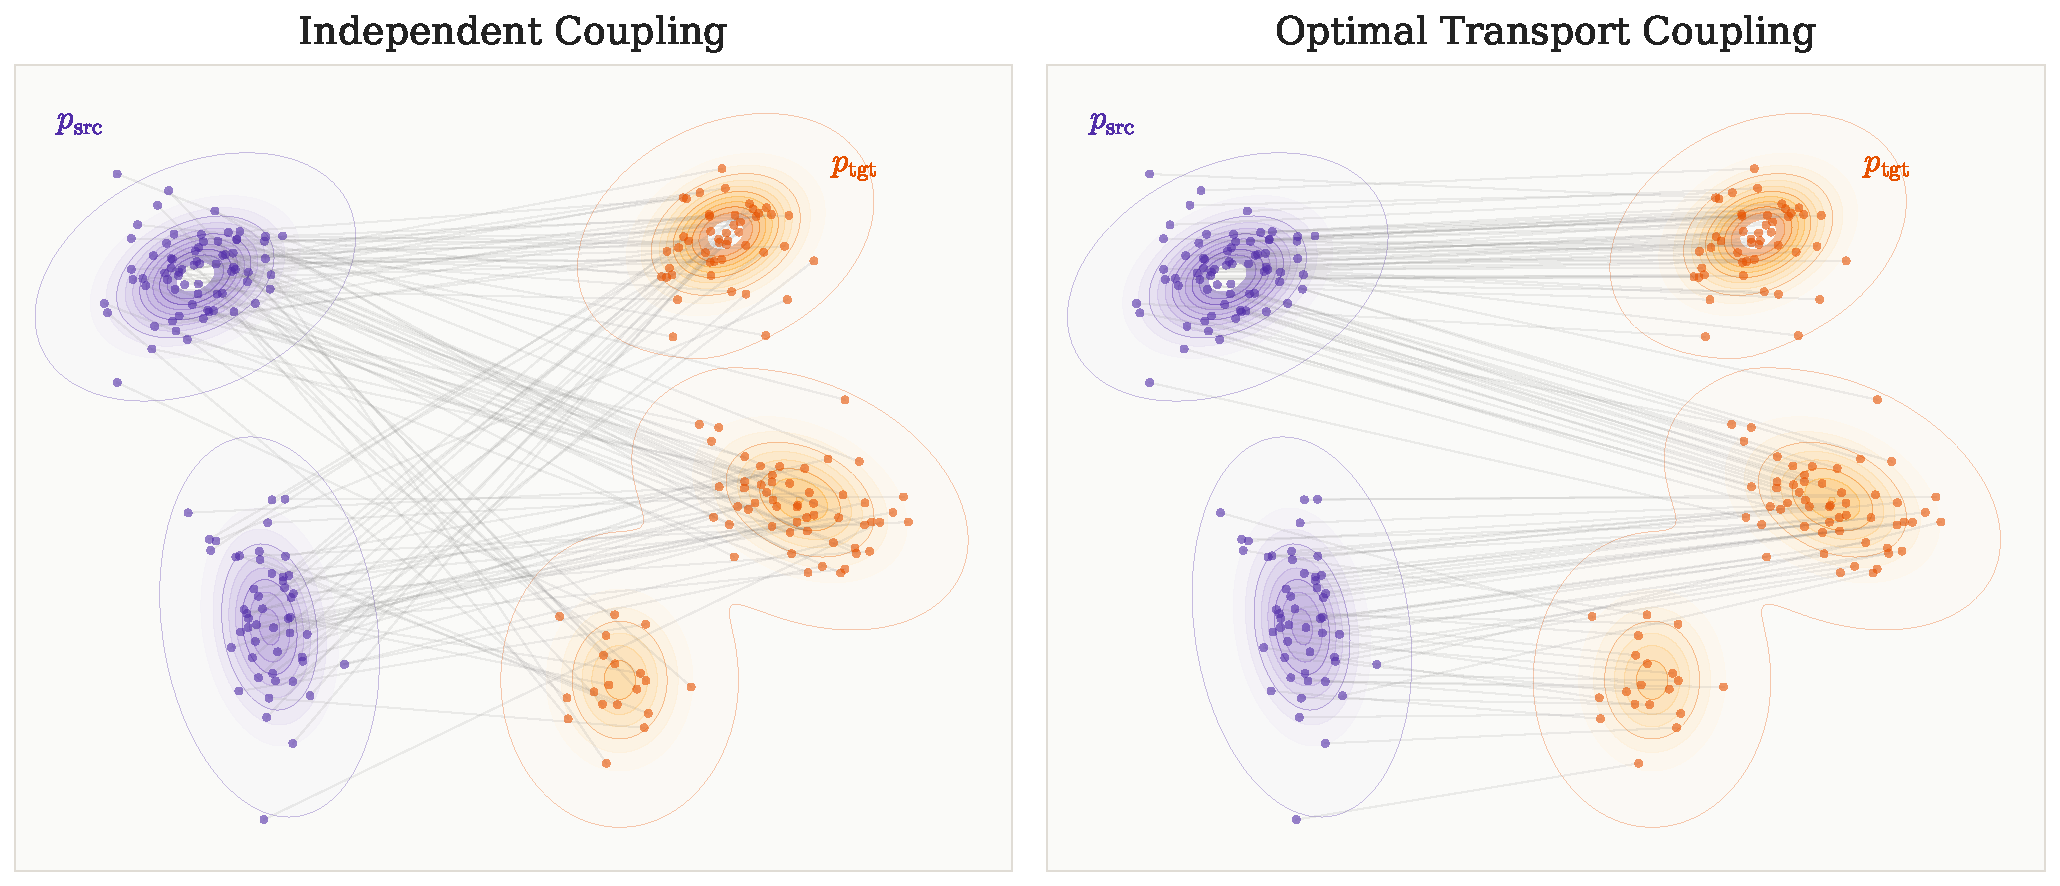
\includegraphics[width=\linewidth]{Images/PartB/ot_2d_coupling_comparison.pdf}
    \caption{\textbfs{同一对二维分布 $p_{\mathrm{src}}$ 和 $p_{\mathrm{tgt}}$ 的两种耦合。}
    左：独立（随机）配对会产生代价高昂的交叉路径。右：最优传输耦合把邻近的质量配对，从而避免交叉。
    \figcredit{由作者使用人工智能辅助编码创建。}}
    \label{fig:ot-2d-coupling}
\end{figure}

\paragraph{Monge--Kantorovich（静态）表述的 OT 问题。}
固定一个代价函数 $c:\R^D\times\R^D\to\R$，它刻画把概率质量从 $\rvx$ 送到 $\rvy$ 所需的花费。我们的目标是尽可能便宜地把源分布 $p_{\mathrm{src}}$ 变换成目标分布 $p_{\mathrm{tgt}}$。

要定义代价，首先得知道哪些点对 $(\rvx,\rvy)$ 被配对在一起。承担这一角色的是
\emph{耦合（coupling）}：定义在 $\R^D\times\R^D$ 上的一个联合分布 $\gamma$，其两个边缘分布分别为
$p_{\mathrm{src}}$ 与 $p_{\mathrm{tgt}}$。换句话说，从 $\gamma$ 中采样 $(\rvx,\rvy)\sim\gamma$，就意味着把源中的一个 $\rvx$ 与目标中的一个 $\rvy$ 配成一对。若 $\gamma$ 关于勒贝格测度存在密度 $\gamma(\rvx,\rvy)$，则边缘约束可写成
\[
\int_{\R^D} \gamma(\rvx,\rvy)\,\diff \rvy = p_{\mathrm{src}}(\rvx),
\qquad
\int_{\R^D} \gamma(\rvx,\rvy)\,\diff \rvx = p_{\mathrm{tgt}}(\rvy).
\]
也就是说，对 $\rvy$ 积分可以把源分布在 $\rvx$ 处的密度还原出来，而对 $\rvx$ 积分则把目标分布在 $\rvy$ 处的密度还原出来。下面给出两个标准例子加以说明：
\begin{enumerate}
    \item \textbfs{离散支撑。}
    如果 $p_{\mathrm{src}}$ 与 $p_{\mathrm{tgt}}$ 都只支撑在有限多个点上，则耦合可用一个非负矩阵 $(\gamma_{ij})$ 表示，其行和等于 $p_{\mathrm{src}}(i)$、列和等于 $p_{\mathrm{tgt}}(j)$。每个元素 $\gamma_{ij}$ 就是从 $i$ 送往 $j$ 的质量。
    \item \textbfs{确定性映射。}
    如果存在可测量的映射 $\rmT$ 与 $\rmT_\#p_{\mathrm{src}}=p_{\mathrm{tgt}}$，那么
    $\gamma=(\rmI,\rmT)_\#p_{\mathrm{src}}$ 是移动每个点的确定性耦合
    $\rvx$ 直接到 $\rmT(\rvx)$.
\end{enumerate}

一旦固定了耦合 $\gamma$，传输代价就是该配对方案下单位代价的期望值：
\[
\int c(\rvx,\rvy)\,\diff\gamma(\rvx,\rvy)
=\E_{(\rvx,\rvy)\sim\gamma}\!\big[c(\rvx,\rvy)\big].
\]
在离散情形下它退化为 $\sum_{i,j} c_{ij}\gamma_{ij}$，而在连续情形下它是一个二重积分。以下我们只讨论连续情形。

于是最优传输问题就是：在所有允许的耦合中，挑出使该期望代价最小的那一个。
\begin{mdframed}
\begin{equation}\label{eq:ot}
\mathrm{OT}\big(p_{\mathrm{src}},p_{\mathrm{tgt}}\big)
:= \inf_{\gamma\in\Gamma(p_{\mathrm{src}},p_{\mathrm{tgt}})}
\int c(\rvx,\rvy)\,\diff\gamma(\rvx,\rvy),
\end{equation}
\end{mdframed}
其中可行集仅强制执行边缘或质量守恒约束：
\begin{align*}
    \Gamma(p_{\mathrm{src}},p_{\mathrm{tgt}})
= \Big\{\gamma \in &\mathcal{P}(\R^D\times\R^D): \\
&\int \gamma(\rvx,\rvy) \diff \rvy = p_{\mathrm{src}}(\rvx),\,\,
\int \gamma(\rvx,\rvy)\diff \rvx = p_{\mathrm{tgt}}(\rvy)\Big\},
\end{align*}
其中 $\mathcal{P}(\R^D\times\R^D)$ 表示 $\R^D\times\R^D$ 上所有概率测度构成的集合。


\subparagraph{特例：Wasserstein-2 距离。}

Wasserstein-2 距离是具有二次成本的 Monge--Kantorovich 问题的特例 $c(\mathbf{x}, \mathbf{y}) = \|\mathbf{x} - \mathbf{y}\|^2$。它测量两个概率分布之间的距离，如下所示：
\begin{align*}
 \mathcal{W}_2^2(p_{\mathrm{src}}, p_{\mathrm{tgt}}) := \inf_{\gamma \in \Gamma(p_{\mathrm{src}}, p_{\mathrm{tgt}})} \mathbb{E}_{(\mathbf{x}, \mathbf{y}) \sim \gamma} \left[ \|\mathbf{x} - \mathbf{y}\|^2 \right].
\end{align*}在关于 $p_{\mathrm{src}}$ 与 $p_{\mathrm{tgt}}$ 的适当假设下，Brenier 定理（见 \Cref{thm:brenier}）\footnote{Brenier 定理讨论二次代价下最优传输映射的存在性与结构。具体而言，若 $p_{\mathrm{src}}$ 不给任何维数至多为 $D-1$ 的集合分配质量，则最优传输映射 $\rmT^*$ 存在且唯一。} 保证二次代价下的最优耦合 $\gamma$ 集中在一个确定性映射 $\rmT:\mathbb{R}^D \rightarrow \mathbb{R}^D$ 的图像上。因此，Wasserstein-2 距离也可以等价地写成\footnote{$\mathcal{W}_2$ 距离有三种常用表述：Monge 表述（基于最优传输映射）、Kantorovich 表述（基于耦合）以及 Benamou--Brenier 动态表述（见 \Cref{eq:bb-ot}）。在适当的正则性条件下，三者相互等价。}：
\begin{equation}\label{eq: Monge's Formulation}    \mathcal{W}_2^2(p_{\mathrm{src}}, p_{\mathrm{tgt}}) = \inf_{\substack{\rmT:\mathbb{R}^D \rightarrow \mathbb{R}^D,\\ \text{ s.t. }\rmT\#p_{\mathrm{src}} = p_{\mathrm{tgt}}}} \mathbb{E}_{\rvx \sim p_{\mathrm{src}}} \left[ \| \rmT(\rvx) - \rvx \|^2 \right].
\end{equation}
这里 $\rmT\#p_{\mathrm{src}} = p_{\mathrm{tgt}}$ 表示 $\rmT$ 把 $p_{\mathrm{src}}$ 前推到 $p_{\mathrm{tgt}}$，即当 $\rvx \sim p_{\mathrm{src}}$ 时 $\rmT(\rvx) \sim p_{\mathrm{tgt}}$。

由此可见，Wasserstein-2 距离衡量的是：在所有与给定边缘分布相匹配的耦合或传输映射中，期望平方传输代价可以取到的最小值。使该最小值取到的传输映射 $\rmT^*(\mathbf{x})$（称为 \emph{Monge 映射}），给出了把 $p_{\mathrm{src}}$ 变换为 $p_{\mathrm{tgt}}$ 的最有效方式。

\paragraph{Benamou--Brenier 的动态最优传输表述。}
\begin{figure}[th!]
    \centering
    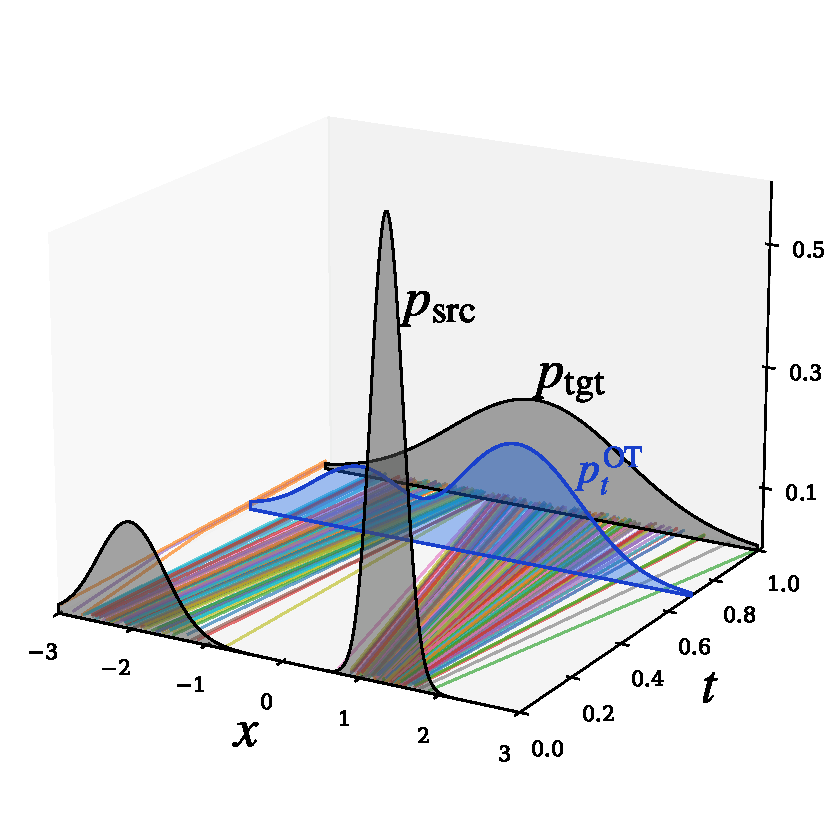
\includegraphics[width=0.8\linewidth]{Images/PartB/ot_illustration.pdf}
    \caption{\textbfs{OT 的动态视角图解。} 插值 $p_t^{\mathrm{OT}}$ 随时间不断演化，
给出以确定性映射实现最低代价的传输方案
（从 $p_{\mathrm{src}}$ 到 $p_{\mathrm{tgt}}$ 的 McCann 位移插值）。
\figcredit{由作者绘制。}}
    \label{fig:ill-ot}
\end{figure}


除了像 Monge--Kantorovich 表述那样直接给出静态的分布对应关系，传输也可以建模为一条连续时间流：
\begin{equation*}
    p_0 := p_{\mathrm{src}} \to p_t \to p_1 := p_{\mathrm{tgt}}, \quad t \in [0,1].
\end{equation*}
\citet{benamou2000computational} 提出的最优传输动态表述，其做法是寻找一个光滑的速度场 $\rvv_t(\rvx)$，用它描述 $p_t(\rvx)$ 中的质量随时间如何演化。

Benamou--Brenier 公式\footnote{Benamou--Brenier 公式说明：$W_2$ 距离可以通过在「测度—速度」的连续路径上最小化动能来计算。} 表明，对于二次代价 $c(\rvx, \rvy) = \|\rvx - \rvy\|_2^2$（即 $\mathcal{W}_2$ 距离），\Cref{eq:ot} 中静态 OT 问题的最优值等于下面这个动能最小化问题的最优值：

\begin{mdframed}
   \begin{equation}\label{eq:bb-ot}
    \mathcal{W}_2^2(p_{\mathrm{src}}, p_{\mathrm{tgt}}) = \min_{\substack{ (p_t, \rvv_t) \text{ s.t. }
        \partial_t p_t + \nabla \cdot (p_t \rvv_t) = 0, \\
        p_0 = p_{\mathrm{src}},\,\, p_1 = p_{\mathrm{tgt}}
    }}
    \int_0^1 \int_{\mathbb{R}^D} \|\rvv_t(\rvx)\|^2 p_t(\rvx) \diff\rvx \diff t
\end{equation}
\end{mdframed}
其中对每个 $t \in [0,1]$，$p_t$ 都是 $\mathbb{R}^D$ 上的概率分布。特别地，最优传输流 $p_t(\rvx)$ 具有如下形式，称为 \textit{McCann 位移插值}：
\begin{equation*}
    \rmT_t^*(\rvx) = (1 - t)\rvx + t\rmT^*(\rvx),
\end{equation*}
其中 $\rmT^*(\rvx)$ 是把 $p_{\mathrm{src}}$ 传输到 $p_{\mathrm{tgt}}$ 的 OT 映射。这一线性插值以恒定速度沿直线搬运质量：对每个 $t \in [0,1]$ 都有 $p_t = \rmT_t^*\#p_{\mathrm{src}}$。最优传输映射 $\rmT^*$ 满足 \emph{Monge--Ampère 方程}：

\begin{equation}\label{eq:monge-ampere}
    p_{\mathrm{tgt}}\left(\nabla \psi(\rvx)\right) \det\left(\nabla^2 \psi(\rvx)\right) = p_{\mathrm{src}}(\rvx),
\end{equation}
其中按 Brenier 定理，$\rmT^*(\rvx) = \nabla \psi(\rvx)$ 对某个凸函数 $\psi$ 成立。然而，这个非线性偏微分方程通常很难求出显式解。值得注意的是，这正是归一化流所用的变量替换关系（见 \Cref{eq:nf-change-of-var}）：归一化流借助易于计算的雅可比行列式来参数化可逆传输映射，但一般并不强加势函数的梯度结构 $\rmT^*=\nabla\psi$；因此训练出来的流可能与 Brenier/OT 映射相差甚远。


\subsection{熵正则最优传输 (EOT)}

为具体说明 EOT 的动因，先考虑由样本构造的经验分布。设 $p_{\mathrm{src}}$ 支撑在点集 $\{\rvx^{(i)}\}_{i=1}^n \subset \R^D$ 上、权重为 $a_i$，而 $p_{\mathrm{tgt}}$ 支撑在 $\{\rvy^{(j)}\}_{j=1}^n \subset \R^D$ 上、权重为 $b_j$。此时耦合就是一个 $n\times n$ 的非负矩阵 $\gamma=(\gamma_{ij})$，其行和与 $a$ 吻合、列和与 $b$ 吻合。每个元素 $\gamma_{ij}$ 表示从 $\rvx^{(i)}$ 送往 $\rvy^{(j)}$ 的质量\footnote{经验（离散）测度为连续分布提供了一个有原则的代理。当基础代价形如 $c(x,y)=d(x,y)^p$（从而 OT 值等于 $W_p^p$）、且测度具有有限的 $p$ 阶矩时，经验测度会以定量速率收敛到总体 $W_p$；参见 \citet{fournier2015rate} 以及综述 \citet{peyre2019computational}。}。

\paragraph{为什么要规范 OT？}
在这种离散设定下，经典 OT（即把连续表述中的测度取为计数测度，见 \Cref{eq:ot}）退化为最小化
\[
\min_{\gamma=(\gamma_{ij})}\sum_{i,j} C_{ij}\,\gamma_{ij},
\]
其中极小化在所有可行耦合 $\gamma=(\gamma_{ij})$ 上进行，$C_{ij} = c(\rvx^{(i)},\rvy^{(j)})$ 是把一个单位质量从源点 $\rvx^{(i)}$ 搬到目标点 $\rvy^{(j)}$ 的代价，$c:\R^D\times\R^D\to\R_{\ge 0}$ 为给定的基础代价（例如 $c(\rvx,\rvy)=\|\rvx-\rvy\|_2^2$）。

出现两个主要问题：
\begin{enumerate}
    \item \textbfs{非唯一且不稳定。} 极小元 $\gamma^*$ 未必唯一。例如，当两个运输方案达到同样的最低代价时，求解器可以任选其中一个。于是输入 $(a,b,C)$ 的微小变化（比如样本移动、权重微调或代价的轻微扰动）就可能导致解发生跳变。
    \item \textbfs{计算代价高。} 该问题是一个含 $n^2$ 个变量、$2n$ 个约束的线性规划。实用求解器（如匈牙利算法~\citep{kuhn1955hungarian,munkres1957algorithms}、网络单纯形法~\citep{peyre2019computational}）的复杂度通常随 $n$ 以 $\mathcal{O}(n^3)$ 增长，当 $n$ 较大时难以承受。
\end{enumerate}

为突破这些瓶颈，EOT 在经典 OT 目标中引入一个正则项，由参数 $\varepsilon > 0$ 控制强度：
\begin{mdframed}
    \begin{align}\label{eq:eot-epsilon}
\begin{aligned}
        \text{EOT}_\varepsilon(p_{\mathrm{src}}, p_{\mathrm{tgt}}) &:= \min_{\gamma \in \Gamma(p_{\mathrm{src}}, p_{\mathrm{tgt}})} \int c(\rvx,  \rvy)  \diff\gamma(\rvx, \rvy)
        + \varepsilon \mathcal{D}_{\text{KL}}\left(\gamma \Vert M \right).
\end{aligned}
\end{align}
\end{mdframed}
参考测度 $M$ 通常取为两个边缘分布的乘积 $p_{\mathrm{src}} \otimes p_{\mathrm{tgt}}$。KL 散度项与传输方案 $\gamma$ 的香农熵直接相关：
\[
\mathcal{D}_{\text{KL}}(\gamma \,\Vert\, p_{\mathrm{src}} \otimes p_{\mathrm{tgt}}) = -\mathcal{H}(\gamma) + \text{Constant},
\]
其中 $\mathcal{H}(\gamma) := -\int \gamma(\rvx, \rvy) \log \gamma(\rvx, \rvy) \diff \rvx \diff \rvy$。加入这一正则项会带来若干理论与实践上的好处，下面简要说明：
\paragraph{熵正则化为什么有用？}
\begin{enumerate}
  \item \textbfs{解更分散。}
  由于 $t\mapsto t\log t$ 是凸函数且在 $t$ 较大时增长很快，最小化 $\int \gamma\log\gamma$
  会惩罚\emph{尖峰式}的耦合（即某些 $\gamma(\rvx,\rvy)$ 很大、其余接近零的耦合）。在总质量固定为 $\int \gamma=1$ 的前提下，它倾向于让方案 $\gamma(\rvx,\rvy)$ 在 $(\rvx,\rvy)\in\mathbb{R}^D\times\mathbb{R}^D$ 上分布得更均匀。换言之，最大化香农熵会带来更高的「不确定性」（即更强的扩散性）。

  \item \textbfs{严格凸性与唯一性。}
  由于 $\mathcal{H}$ 严格凹，\Cref{eq:eot-epsilon} 中的目标函数关于 $\gamma$ 严格凸，从而给出\emph{唯一}的极小元 $\gamma^*_\varepsilon$，且它连续地依赖于 $(p_{\mathrm{src}},p_{\mathrm{tgt}},c)$。

  \item \textbfs{Sinkhorn 形式与严格正性。}
  在适当条件下\footnote{我们假定 $c<\infty$ 在 $p_{\mathrm{src}}\otimes p_{\mathrm{tgt}}$-几乎处处的意义下成立，且关于各边缘分布的核积分有限且为正。为简洁起见，我们主要考虑 $\gamma^*_\varepsilon$、$p_{\mathrm{src}}$ 与 $p_{\mathrm{tgt}}$ 均关于勒贝格测度存在密度的情形。}，极小元具有如下的\emph{薛定谔/Sinkhorn 形式}：
  \[
  \gamma^*_\varepsilon(\rvx,\rvy) = u(\rvx)\, \exp \bigl(-\tfrac{c(\rvx,\rvy)}{\varepsilon}\bigr)  \,v(\rvy)p_{\mathrm{src}}(\rvx) p_{\mathrm{tgt}}(\rvy),
  \]
  其中 $u,v$ 为正的缩放函数（在整体意义下唯一）。实践中，连续表述用有限样本做近似，EOT 于是化为有限（采样）的 Sinkhorn 迭代。熵目标严格凸，可用缩放类算法（Sinkhorn/IPFP）高效求解~\citep{sinkhorn1964relationship,cuturi2013sinkhorn}。若每条边缘有 $n$ 个支撑点（即 $n\times n$ 的核矩阵），每次 Sinkhorn 迭代只需 $\mathcal{O}(n^2)$ 的时间与 $\mathcal{O}(n^2)$ 的内存，这使得该方法更具可扩展性、也更为实用~\citep{altschuler2017near}。

  \item \textbfs{对 $\varepsilon$ 的极限行为。}
当 $\varepsilon \to 0$ 时，最优方案 $\gamma^*_\varepsilon$ 越来越集中，趋近于（可能不唯一的）经典 OT 耦合（详见 \Cref{subsec:eot-ot}）。随着 $\varepsilon$ 增大，$\gamma^*_\varepsilon$ 逐渐铺开，并趋近于独立耦合 $p_{\mathrm{src}}\otimes p_{\mathrm{tgt}}$。
\end{enumerate}


\subsection{薛定谔桥 (SB)}\label{subsec:sb}


\paragraph{SB 的 KL 表述。}
薛定谔桥（SB）问题由 Erwin Schrödinger 于 20 世纪 30 年代提出，问的是这样一件事。设想粒子按某个简单的参考动力学运动，例如布朗运动。现在我们只在两个时刻观测粒子：$t=0$ 时其分布为 $p_{\mathrm{src}}$，$t=1$ 时其分布为 $p_{\mathrm{tgt}}$。在连接这两个分布的所有可能的随机过程中，哪一个与参考动力学的偏离最小？这里的「偏离」用 KL 散度度量，因此 SB 问题的解，就是把布朗运动扭曲成满足指定边界条件的过程时最可能的那个变形方式。

为把这一点说清楚，令 $\rvx_{0:T}:=\{\rvx_t\}_{t\in[0,T]}$ 表示过程的完整轨迹。用 $P$ 记\emph{轨迹律}，即整条样本路径上的概率分布。$P$ 在时刻 $t$ 的边缘分布记为 $p_t$（或 $P_t$），它描述某个时刻 $t$ 的状态 $\rvx_t$ 的分布。形式上，对任意可测集 $A\subseteq\mathbb R^D$，
\[
p_t(A) = P(\rvx_t \in A).
\]
换言之，$p_t$ 可以看作：采样许多条完整轨迹后，把每条轨迹在时刻 $t$ 的状态收集起来所得的经验分布——例如当状态是一维时，它就是一个直方图。


考虑由如下 SDE 驱动的参考扩散 $\{\rvx_t\}_{t\in[0,T]}$：
\begin{align}\label{eq:general-sb-sde}
    \diff \rvx_t  =  \rvf(\rvx_t,t)\,\diff t  +  g(t)\,\diff \rvw_t,
\end{align}
其中 $\rvf\colon \R^D\times[0,T]\!\to\!\R^D$、$g\colon[0,T]\!\to\!\R$，而
$\{\rvw_t\}_{t\in[0,T]}$ 是标准布朗运动。用 $R$ 表示整条轨迹
$\rvx_{0:T}:=\{\rvx_t\}_{t\in[0,T]}$ 的\emph{路径律}（即其联合分布），$R_0$ 表示参考过程的初始边缘分布；这个 $R$ 就充当\emph{参考}轨迹分布。有了这套记号，SB 问题就是在 KL 散度意义下寻找与 $R$ 最接近、同时满足给定端点边缘约束的轨迹律 $P$：
\begin{align}\label{eq:sb-epsilon-general}
    \mathrm{SB}(p_{\mathrm{src}}, p_{\mathrm{tgt}})
    := \min_{P}\, \mathcal{D}_{\mathrm{KL}}(P\|R)
    \quad \text{s.t.} \quad P_0 = p_{\mathrm{src}},\;\; P_T = p_{\mathrm{tgt}}.
\end{align}
其最优解 $P^*$ 依赖于所选取的参考过程 $R$。

\paragraph{SB 的随机控制视图。}

\begin{figure}[th!]
    \centering
    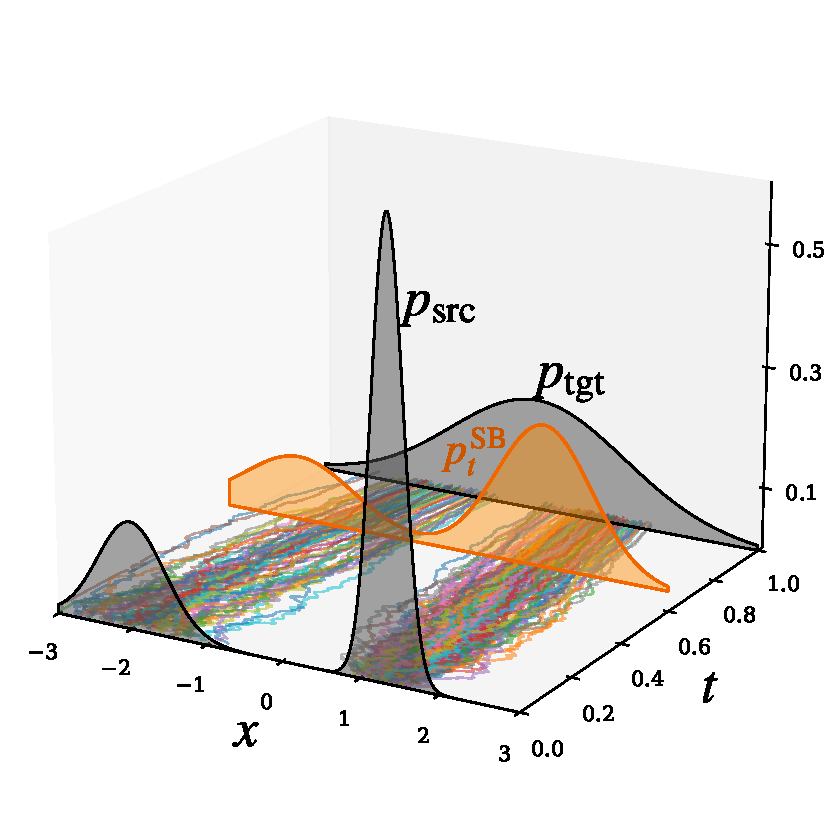
\includegraphics[width=0.75\linewidth]{Images/PartB/sb_illustration.pdf}
    \caption{\textbfs{SB 的随机控制视角图解。} 桥问题要寻找一条在连接 $p_{\mathrm{src}}$ 与 $p_{\mathrm{tgt}}$ 的同时、偏离参考动力学最小的随机路径。
    \figcredit{由作者绘制。}}
    \label{fig:ill-sb}
\end{figure}


与其在 \Cref{eq:sb-epsilon-general} 中直接对任意的路径分布 $P$ 做优化，一种更易处理的做法是把参考动力学当作锚点，然后允许它发生漂移：引入一个依赖时间的漂移项 $\rvv_t(\rvx_t)$ 去扰动参考过程，由此生成一族候选的轨迹分布。于是得到的动力学就是一个\emph{受控扩散}：
\[
    \diff \rvx_t
    = \bigl[\rvf(\rvx_t,t) + \rvv_t(\rvx_t)\bigr]\diff t + g(t) \diff \rvw_t,
\]
其中 $\rvv_t:\R^D\to\R^D$ 就是待优化的漂移（见 \Cref{eq:sb-kinetic}）。在标准的可积性条件（例如 Novikov 条件）以及 Girsanov 定理（见 \Cref{subsec:girsanov}）之下，受控律 $P$ 与参考律 $R$ 之间的 KL 散度可写成如下的动力学（kinetic）形式
\begin{align*}
    \mathcal{D}_{\mathrm{KL}}(P\|R)
    &=
    \mathcal{D}_{\mathrm{KL}}(p_{\mathrm{src}}\|R_0)
    +
    \E_{P}\!\left[
    \frac{1}{2}\int_0^T
    \frac{\|\rvv_t(\rvx_t)\|^2}{g^2(t)}
    \diff t
    \right]
    \\
    &=
    \mathcal{D}_{\mathrm{KL}}(p_{\mathrm{src}}\|R_0)
    +
    \frac{1}{2}\int_0^T\!\int_{\R^D}
    \frac{\|\rvv_t(\rvx)\|^2}{g^2(t)}
    p_t(\rvx)\diff\rvx\diff t .
\end{align*}
其中 $p_t$ 是受控过程下 $\rvx_t$ 的 $t$-时刻边缘分布。第二个等式由全期望公式得到。由于 SB 问题中 $P_0=p_{\mathrm{src}}$ 是固定的，第一项对控制而言是常数，因而可在优化中省去；特别地，当 $R_0=p_{\mathrm{src}}$ 时它直接为零。因此，SB 问题可以重新表述为：在所有允许的漂移中，最小化引导该过程的期望控制能量 $\rvv_t$
$p_{\mathrm{src}}$ 在 $t=0$ 至 $p_{\mathrm{tgt}}$ 在 $t=T$
\citep{dai1991stochastic,pra1990markov,pavon1991free,chen2016relation}。由于初始边缘固定为 $p_{\mathrm{src}}$，我们可以参考流程有 $R_0=p_{\mathrm{src}}$ 不改变优化器；然后
$\mathcal{D}_{\mathrm{KL}}(p_{\mathrm{src}}\|R_0)=0$。这导致 \emph{随机控制公式}:
\begin{mdframed}
\begin{align}\label{eq:sb-kinetic}
\begin{aligned}
\mathrm{SB}(p_{\mathrm{src}}, p_{\mathrm{tgt}})
=
\min_{\substack{
\mathbf{v}_t \text{ s.t. }
\diff \rvx_t =
\left[\rvf(\rvx_t,t)+\mathbf{v}_t(\rvx_t)\right]\diff t
+g(t)\diff\rvw_t,\\
\rvx_0\sim p_{\mathrm{src}},\,
\rvx_T\sim p_{\mathrm{tgt}}
}}
\frac{1}{2}
\int_0^T\int_{\mathbb{R}^D}
\frac{\norm{\rvv_t(\rvx)}^2}{g^2(t)}
p_t(\rvx)\diff\rvx\diff t .
\end{aligned}
\end{align}
\end{mdframed}
要注意，端点分布 $p_{\mathrm{src}}$ 与 $p_{\mathrm{tgt}}$ 是任意给定的；而控制量 $\rvv_t$ 正是为了在这两个边缘之间「架桥」——在把参考动力学接到两端的同时，尽量（在 KL 散度意义上）贴近参考过程 $R$。

\paragraph{布朗运动作为特殊的参考过程。}
\Cref{eq:sb-kinetic} 与 OT 中的 Benamou--Brenier 公式 \Cref{eq:bb-ot} 形式相似，尤其是当参考过程
$R^\varepsilon$（$\varepsilon>0$）取为布朗运动时\footnote{这种相似性还可以说得更精确。在等价的时间对称流体动力学表述中，若用 $\tilde{\rvv}_t$ 表示满足连续性方程
$\partial_t \rho_t + \nabla \cdot (\rho_t \tilde{\rvv}_t)=0$ 的当前速度，则布朗参考下的 SB 目标（\Cref{eq:sb-epsilon-kinetic}）可写成 Benamou--Brenier 型的动力学项（只差一个常数因子）再加上一个 Fisher 信息项：
\[
\int_0^T\!\!\int
\left[
\frac{1}{2}\|\tilde{\rvv}_t(\rvx)\|^2
+
\frac{\varepsilon^2}{8}\|\nabla_{\rvx}\log \rho_t(\rvx)\|^2
\right]\rho_t(\rvx)\,\diff\rvx\,\diff t.
\]
因此，在布朗参考、二次代价的情形下，熵 OT 可以看作动态 OT 的 Fisher 信息正则化版本；见 \citet{chen2021stochastic} 中的问题 4.6。}：
\[
\diff \rvx_t = \sqrt{\varepsilon}\,\diff\rvw_t,
\]
此时 $\rvf \equiv \mathbf{0}$、$g(t) \equiv \sqrt{\varepsilon}$。在这一设定下，SB 问题就是在 KL 散度意义下寻找与布朗参考 $R^\varepsilon$ 最接近、同时满足端点边缘约束的路径分布 $P$：
\begin{align}\label{eq:sb-epsilon}
    \mathrm{SB}_\varepsilon(p_{\mathrm{src}}, p_{\mathrm{tgt}})
    := \min_{P} \mathcal{D}_{\mathrm{KL}}(P \| R^\varepsilon)
    \quad \text{s.t.} \quad P_0 = p_{\mathrm{src}}, \;\; P_T = p_{\mathrm{tgt}}.
\end{align}
等价的随机控制表述则变为
\begin{align}\label{eq:sb-epsilon-kinetic}
\begin{aligned}
    \mathrm{SB}_\varepsilon(p_{\mathrm{src}}, p_{\mathrm{tgt}})
    = \min_{\substack{
        \rvv_t \text{ s.t. } \diff \rvx_t = \rvv_t(\rvx_t)\,\diff t + \sqrt{\varepsilon}\,\diff \rvw_t, \\
        \rvx_0 \sim p_{\mathrm{src}},\;\; \rvx_T \sim p_{\mathrm{tgt}}
    }}
    \frac{1}{2\varepsilon}\int_0^T \!\!\int_{\R^D}
        \|\rvv_t(\rvx)\|^2 \, p_t(\rvx)\,\diff \rvx\,\diff t,
\end{aligned}
\end{align}
其中 $p_t$ 表示由漂移 $\rvv_t$ 驱动的扩散过程在时刻 $t$ 的边缘分布：
\[
\diff \rvx_t = \rvv_t(\rvx_t)\,\diff t + \sqrt{\varepsilon}\,\diff \rvw_t.
\]


\paragraph{为什么必须指定参考分布？}
经典 OT 不需要参考路径分布，因为给定的基础代价已经告诉我们把源点与目标点配对要花多少代价，于是优化时直接借助该代价来比较各个允许的耦合即可。但在 SB 问题中，我们比较的是整条随机轨迹，而不只是它们的端点。因此需要一个参考路径测度 $R$，用它指明「不加控制时动力学通常是什么样子」。量
$\mathcal{D}_{\mathrm{KL}}(P\|R)$ 衡量的正是：为了让端点分布符合要求，允许的过程
$P$ 必须偏离这套参考动力学多远。


\paragraph{耦合偏微分方程刻画。}
描述 SB 解的一种便捷方式，是借助两个时空势函数 $\Psi(x,t)$ 与 $\widehat{\Psi}(x,t)$。令
$p_t^{\mathrm{SB}}$ 表示 \Cref{eq:sb-epsilon-general} 中最优轨迹律 $P^*$ 在 $t\in[0,T]$ 时刻的边缘分布，则有如下对称分解~\citep{dai1991stochastic}：
\begin{align}\label{eq:sb-symmetry}
p_t^{\mathrm{SB}}(x) = \Psi(x,t) \widehat{\Psi}(x,t),
\end{align}
其中 $\Psi$ 与 $\widehat{\Psi}$ 求解一个（线性的）\emph{薛定谔系统}~\citep{caluya2021wasserstein,chen2021stochastic,chenlikelihood}：
\begin{align}
\begin{aligned}\label{eq:pde-schrodinger}
\frac{\partial \Psi}{\partial t}(\mathbf{x},t)
  &= -\nabla_{\mathbf{x}} \Psi(\mathbf{x},t) \cdot \rvf(\mathbf{x},t)
     - \frac{g^2(t)}{2}\,\Delta_\mathbf{x} \Psi(\mathbf{x},t),  \\
\frac{\partial \widehat{\Psi}}{\partial t}(\mathbf{x},t)
  &= -\nabla_{\mathbf{x}}\!\cdot\!\bigl(\widehat{\Psi}(\mathbf{x},t)\,\rvf(\mathbf{x},t)\bigr)
     + \frac{g^2(t)}{2}\,\Delta_\mathbf{x}\widehat{\Psi}(\mathbf{x},t)
\\ \text{subject to}\quad
\Psi(\mathbf{x},0)&\,\widehat{\Psi}(\mathbf{x},0) = p_{\mathrm{src}}(\mathbf{x}),
\quad
\Psi(\mathbf{x},T)\,\widehat{\Psi}(\mathbf{x},T) = p_{\mathrm{tgt}}(\mathbf{x}).
\end{aligned}
\end{align}

\iffalse

\begin{align}
\begin{aligned}\label{eq:pde-schrodinger}
\frac{\partial \Psi}{\partial t}(\mathbf{x},t)
  &= -\nabla_{\mathbf{x}} \Psi(\mathbf{x},t)^\top\,\rvf(\mathbf{x},t)
     - \frac{1}{2}\,\mathrm{Tr}\bigl(g^2(t)\,\nabla_{\mathbf{x}}^2\Psi(\mathbf{x},t)\bigr),  \\
\frac{\partial \widehat{\Psi}}{\partial t}(\mathbf{x},t)
  &= -\nabla_{\mathbf{x}}\!\cdot\!\bigl(\widehat{\Psi}(\mathbf{x},t) \rvf(\mathbf{x},t)\bigr)
     + \frac{1}{2} \mathrm{Tr}\bigl(g^2(t)\,\nabla_{\mathbf{x}}^2\widehat{\Psi}(\mathbf{x},t)\bigr)
\\[4pt] \text{subject to}  \\[4pt]
\Psi(\mathbf{x},0)& \widehat{\Psi}(\mathbf{x},0) = p_{\mathrm{src}}(\mathbf{x}),
\quad
\Psi(\mathbf{x},T) \widehat{\Psi}(\mathbf{x},T) = p_{\mathrm{tgt}}(\mathbf{x}).
\end{aligned}
\end{align}
\fi

\subparagraph{正向时间的薛定谔桥 SDE。}
一旦 $\Psi$ 已知，最优动力学就是以时空因子 $\Psi$ 做倾斜的参考扩散：
\begin{align}\label{eq:sb-forward-sde}
    \diff \rvx_t = \bigl[\rvf(\rvx_t, t) + g^2(t)\,\nabla_{\mathbf{x}} \log \Psi(\rvx_t, t)\bigr]\diff t
+ g(t)\diff \rvw_t, \quad \rvx_0 \sim p_{\mathrm{src}}.
\end{align}
用 $Q$ 表示 \Cref{eq:sb-forward-sde} 的轨迹律
（由 \Cref{eq:sb-symmetry,eq:pde-schrodinger} 可知 $Q_0=p_{\mathrm{src}}$、$Q_T=p_{\mathrm{tgt}}$）。此时
\emph{$Q=P^*$}，而 \Cref{eq:sb-kinetic} 的极小元 $\rvv^*$ 为（参见 \citet{chen2021stochastic} 第 4.6 节）：
\[
\rvv_t^{*}(\rvx) = g^2(t) \nabla_\rvx \log \Psi(\rvx,t).
\]
也就是说，漂移修正项 $g^2\nabla_\rvx\log\Psi$ 正是为了让端点边缘相匹配，对参考过程施加的 KL 意义下最小的扰动。


\subparagraph{反向时间的薛定谔桥 SDE。}
同一条最优路径律也可以在时间上反向生成。要看出反向漂移的形式，一个便捷的做法是概念上套用扩散过程标准的逆时间恒等式：
\[
\rvb^{-}(\rvx,t)=\rvb^{+}(\rvx,t)-g^2(t)\nabla_\rvx\log p_t^{\mathrm{SB}}(\rvx),
\]
其中 $\rvb^{+}=\rvf+g^2\nabla\log\Psi$ 和 $p_t=\Psi\,\widehat{\Psi}$。这给出了
\[
\rvb^{-}(\rvx,t)=\rvf(\rvx,t)-g^2(t) \nabla_\rvx\log \widehat{\Psi}(\rvx,t).
\]
因此反向时间的 SDE 为
\begin{align}\label{eq:sb-backward-sde}
\diff \rvx_t
= \Big[\rvf(\rvx_t,t) - g^2(t) \nabla_{\rvx}\log \widehat{\Psi}(\rvx_t,t)\Big]\diff t
+ g(t)\,\diff \bar{\rvw}_t, \quad \rvx_T \sim p_{\mathrm{tgt}} .
\end{align}
等价地，可以重新参数化时间：令 $\rvy_\tau := \rvx_{T-\tau}$，让
$\tau$ 从 $0$ 递增到 $T$。于是 $\rvy_\tau$ 沿正向的 $\tau$ 演化，初值为 $\rvy_0 \sim p_{\mathrm{tgt}}$，满足
\begin{align}\label{eq:sb-reverse-forward-tau}
\begin{aligned}
    \diff \rvy_\tau
= \big[-\rvf(\rvy_\tau,T-\tau) + g^2(T-\tau) \nabla_{\rvy}\log \widehat{\Psi}(\rvy_\tau,T-\tau)\big]\diff \tau
+ g(T-\tau) \diff \rvw_\tau.
\end{aligned}
\end{align}


正向与反向两种描述给出的是同一条最优路径律 $P^*$，二者通过如下关系相联系：
\[
\nabla\log p_t^{\mathrm{SB}}=\nabla\log\Psi+\nabla\log\widehat\Psi,
\qquad
\rvb^{-}=\rvb^{+}-g^2\,\nabla\log p_t^{\mathrm{SB}},
\]
因此二者在每个时刻 $t$ 的边缘分布都等于 $p_t^{\mathrm{SB}}$。那两个附加漂移项——正向的 $g^2\nabla\log\Psi$ 与反向的 $-\,g^2\nabla\log\widehat{\Psi}$——起控制力的作用，引导参考扩散去匹配端点边缘，同时使相对熵意义下与参考过程的偏离最小。


\subparagraph{耦合偏微分方程方法的实际障碍。}
要按 \Cref{eq:sb-backward-sde} 构造生成过程，必须先求解耦合偏微分方程 \Cref{eq:pde-schrodinger} 以得到反向薛定谔势 $\widehat{\Psi}$。然而，即便在低维情形下，这些偏微分方程也极难求解，这使它们很难直接用于生成建模。为绕过这一困难，已有工作提出了多种替代策略：借用 Score SDE 技术交替求解两个半桥问题（$p_{\mathrm{src}} \to p_{\mathrm{tgt}}$ 与 $p_{\mathrm{tgt}} \to p_{\mathrm{src}}$）~\citep{de2021diffusion}；优化替代的似然界~\citep{chenlikelihood, liu20232}；或者利用后验分布的解析解，为样本对 $(\rvx_0, \rvx_T) \sim p_{\mathrm{src}} \otimes p_{\mathrm{tgt}}$ 设计免模拟的训练目标 $\rvx_t \vert \rvx_0, \rvx_T$~\citep{liu20232}。这里我们不再深入技术细节，而只简要讨论扩散模型与 SB 之间的联系，见 \Cref{sec:dm-and-sb}。

\subsection{全局推前与局部动力学：DGM 的 OT 类比}
从最优传输的角度看（见 \Cref{eq:ot}），我们可以用深度生成模型从简单的先验中学习一个传输（前推）映射，即
$\rmG_{\bm{\phi}\#}p_{\mathrm{prior}} \approx p_{\mathrm{data}}$。虽然 $\rmG_{\bm{\phi}}$ 一般并不等于最优传输映射（除非在适当条件下显式施加 OT 目标的那类工作~\citep{genevay2018learning,onken2021ot}），但 Benamou--Brenier 公式（见 \Cref{eq:bb-ot}）提供了一个互补的、动态的视角：它不直接学一个全局映射，而是把传输描述为由依赖时间的局部向量场生成的连续流，从而在 $p_{\mathrm{prior}}$ 与 $p_{\mathrm{data}}$ 之间描出一条光滑路径。这一动态表述与静态的薛定谔桥问题（见 \Cref{eq:sb-epsilon-general}）以及其随机控制对应形式（见 \Cref{eq:sb-kinetic}）相呼应——在后两者中，最优耦合是由受控扩散过程实现的。生成模型中也有类似的对照：GAN、VAE 等标准深度生成模型学习的是全局前推映射，而扩散模型学习的是驱动生成动力学的、依赖时间的局部向量场。


\section{不同最优传输表述之间的关系}\label{sec:relation-ot}

\begin{figure}[ht!]
\centering

\resizebox{\textwidth}{!}{
\begin{tikzpicture}[
    node distance=2.2cm and 1.2cm,  % <-- REDUCED spacing
    block/.style={
        rectangle, draw, thick, rounded corners,
        fill=white!10, text width=13em,   % <-- REDUCED text width
        minimum height=5em, align=center, font=\normalsize % <-- CHANGED font to normalsize
    },
    arrow/.style = {ultra thick, -{Stealth[length=4mm, width=4mm]}},
    dashed_arrow/.style={-Latex, ultra thick, dashed, color=gray, -{Stealth[length=4mm, width=4mm]}},
    label/.style={midway, font=\small, align=center}
]

% Nodes
\node[block, text width=11em] (sde) {
    {\large \textbfs{SB}$_\varepsilon$ \\ \textbfs{(Stochastic Control)}}\\[0.6em]
See \Cref{eq:sb-epsilon-kinetic}.
};

\node[block, text width=11em, below=of sde] (ode) {
   {\large \textbfs{OT} \\ \textbfs{(Dynamic Formulation)}
   \\ [0.5em]
See \Cref{eq:bb-ot}.
   }
};

\node[block, text width=11em, right=of sde, xshift=1.5cm] (sb) {
    {\large \textbfs{SB}$_\varepsilon$ \\ \textbfs{(Path-Space Formulation)}}\\[0.5em]
$\displaystyle
\min_{\substack{P :\, P_0 = p_{\rm src} \\ \phantom{P :\, } P_T = p_{\rm tgt}}}
  \mathcal{D}_\mathrm{KL}(P \| R^\varepsilon)
$
};

\node[block, right=of sb, xshift=1.5cm] (eot) {
    {\large \textbfs{EOT}$_\varepsilon$ }\\[0.5em]
    $\displaystyle
        \min_{\gamma \in \Gamma(p_{\rm src}, p_{\rm tgt})}
        \int \norm{\rvx-\rvy}_2^2  \diff\gamma
         + \varepsilon  \mathcal{D}_{\mathrm{KL}}(\gamma \| p_{\rm src} \otimes p_{\rm tgt})
    $

};

\node[block, below=of eot] (ot) {
 {\large \textbfs{OT \\ (Static Formulation)} }\\[0.6em]
    $\displaystyle
        \min_{\gamma \in \Gamma(p_{\rm src}, p_{\rm tgt})}
        \int \norm{\rvx-\rvy}_2^2 \diff\gamma
    $
};

% Arrows using the new 'label' style
\draw[arrow] (sde) -- (ode)
    node[label, left]
    {$\varepsilon \to 0$}
    node[label, right]
    {(iv)};
\draw[arrow,<->] (sde.east) -- (sb.west)
  node[pos=.5, above, text width=9em, align=center, sloped]
    {\footnotesize$p_t = P^*(\rvx_t \in \cdot)$}
  node[pos=.5, below, text width=9em, align=center, sloped]{(i)};
\draw[arrow,<->] (sb.east) -- (eot.west)
  node[pos=.5, above, text width=8em, align=center, sloped]
    {Endpoint projection\\ \footnotesize$\gamma^* = (\rvx_0,\rvx_T)_\# P^*$}
  node[pos=.5, below, text width=9em, align=center, sloped]
    {(ii)};
\draw[arrow] (eot) -- (ot)
    node[label, left]
    {$\varepsilon \to 0$}
    node[label, right]
    {(iii)};
\draw[arrow, <->] (ode) -- ([yshift=0.3cm] ot.west)
    node[label, below]
    {$p_t = \bPsi_t\#\gamma^*$，其中 $\bPsi_t(\rvx,\rvy) = (1-t) \rvx + t \rvy$};

\end{tikzpicture}
}
\caption{\textbfs{在二次代价 $c(\rvx,\rvy)=\|\rvx-\rvy\|_2^2$ 与参考过程 $R^\varepsilon$ 下，各最优传输表述之间的关系。}
图中总结的关系为：(i) 随机控制表述与路径空间 KL 表述 $\mathrm{SB}_\varepsilon$ 相互等价；(ii) 对布朗参考（连同相应的二次代价归一化）而言，把 $\mathrm{SB}_\varepsilon$ 的最优解投影到端点上即得
$\mathrm{EOT}_\varepsilon$；(iii) 当 $\varepsilon\to0$ 时，$\mathrm{EOT}_\varepsilon$ 收敛到静态 OT；(iv) 在适当重新标度的布朗参考下，薛定谔问题当 $\varepsilon\to0$ 时收敛到动态 OT。\figcredit{由作者绘制。}}
\label{fig:ot-dm}
\end{figure}


在深入技术细节之前，先厘清最优传输的各
种表述及其熵正则化版本之间的联系会有帮助。从较高层次看，这些问题彼此关联，可概括为（见 \Cref{fig:ot-dm} 的关系图）：
\begin{enumerate}
    \item[(i)] \textbfs{路径空间 SB $\Longleftrightarrow$ 随机控制 SB。}
    路径空间 KL 表述 $\mathrm{SB}_\varepsilon$ 与其随机控制表述所描述的，是同一个相对于所选参考过程的桥问题（参见 \Cref{subsec:sb}）。

    \item[(ii)] \textbfs{布朗参考 SB $\Longleftrightarrow$ EOT$_\varepsilon$.}
    用于布朗参考
    \[
    \diff \rvx_t=\sqrt{\varepsilon}\,\diff\rvw_t,
    \]
    在相应的二次代价归一化下，由最优 SB 路径律诱导出的端点耦合，正是相应
$\mathrm{EOT}_\varepsilon$ 问题的解（参见 \Cref{subsec:sb-eot}）。\item[(iii)] \textbfs{EOT$_\varepsilon$ $\longrightarrow$ 静态 OT.}
    当 $\varepsilon\to0$ 时，熵正则化的端点耦合问题的解收敛到相应的经典 OT 问题，其最优值也在
    \Cref{subsec:eot-ot} 所讨论的假设下收敛到 OT 值。

    \item[(iv)] \textbfs{SB$_\varepsilon$ $\longrightarrow$ 动态 OT.}
    在相应的小噪声标度下，布朗参考的薛定谔问题当 $\varepsilon\to0$ 时收敛到动态 OT 的 Benamou--Brenier 表述
    （参见 \Cref{subsec:sb-ot}）。
\end{enumerate}


这些关系放在一起，为随机控制、熵正则化与经典 OT 三套框架提供了一个紧凑的整体图景。


\begin{figure}[th!]
    \centering
    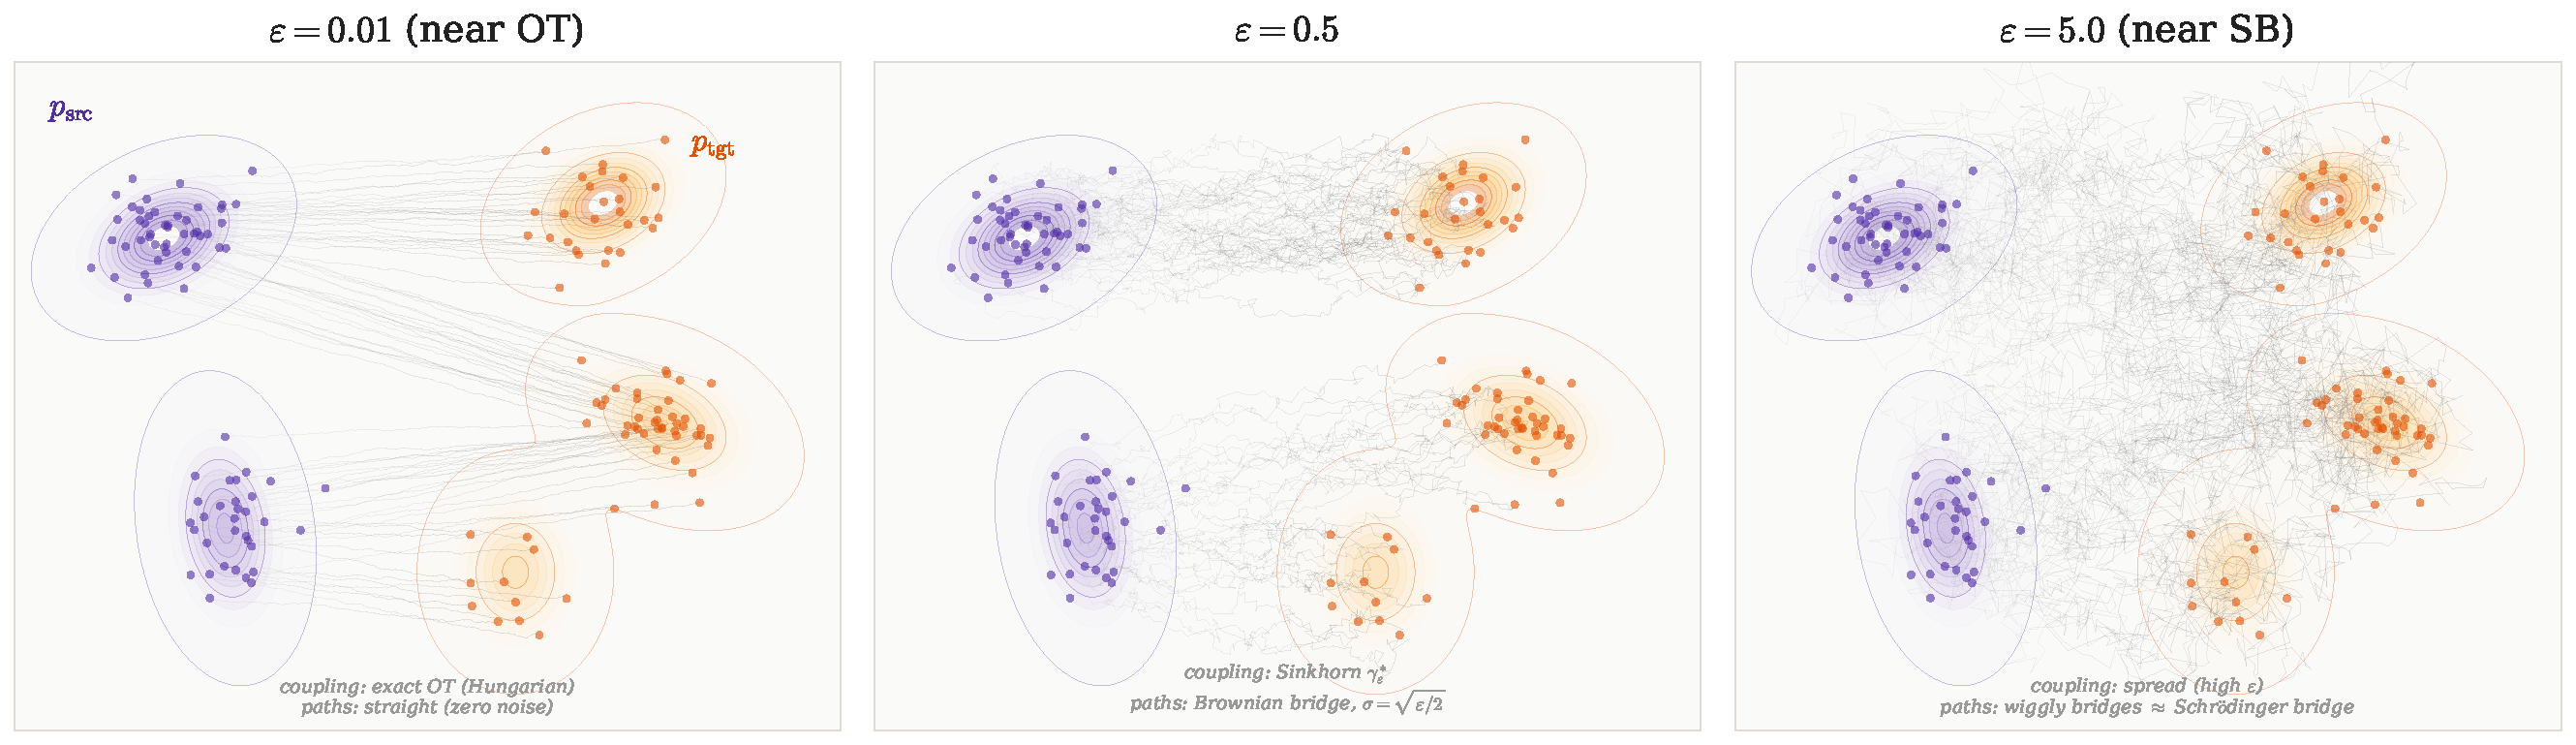
\includegraphics[width=\linewidth]{Images/PartB/eot_epsilon_interpolation.pdf}
    \caption{\textbfs{熵正则参数 $\varepsilon$ 对
    熵最优传输的影响（联系（iii）与（iv））。}
    随着 $\varepsilon$ 增大，有两件事同时发生：
    耦合 $\gamma^*_\varepsilon$ 把质量输送到更远的目标处，
    同时传输路径变得越来越随机。
    左（$\varepsilon=0.01$）：路径几乎是直线，每个源点都被映射到附近的单个目标，回到经典 OT。
    中（$\varepsilon=0.5$）：路径出现明显波动，
    耦合开始扩散。
    右（$\varepsilon=2.5$）：路径高度随机，
    接近薛定谔桥的情形；
    在极限 $\varepsilon\to\infty$ 下，耦合退化为独立乘积
    $p_{\mathrm{src}}\otimes p_{\mathrm{tgt}}$。
    耦合用 Sinkhorn 算法计算
    （$\varepsilon\to 0$ 时即为匈牙利算法）；
    在给定端点的条件下，路径是布朗桥，
    其扩散系数 $\sigma=\sqrt{\varepsilon/2}$，
    可由三上对偶得到（\Cref{subsec:sb-eot}）。
    \figcredit{由作者借助 AI 辅助编码绘制。}}
    \label{fig:eot-epsilon}
\end{figure}

\subsection{SB 与 EOT 的双向等价}\label{subsec:sb-eot}
本节给出两个互补的视角，用以说明 SB 与 EOT 本质上是同一件事。
与经典最优传输给出单个确定性映射不同，SB 产生的是一族\emph{随机}的粒子流：质量以概率方式被传输，其边缘分布在类似扩散的动力学下演化。

从静态角度看，SB 与 EOT 一致，目标都是寻找两个端点分布之间的耦合，以在传输代价与熵之间取得平衡。
从动态角度看，SB 描述的是一族受控扩散过程，它尽可能贴近一个简单的参考过程（例如布朗运动），同时又满足给定的端点分布。这两个视角各自独立地建立了等价性，共同提供两种一致的途径，把 SB/EOT 理解为分布到分布变换的典范表述。

\paragraph{静态薛定谔桥。}
让
\[
  \widetilde R^\varepsilon(\rvx,\rvy)
  := \frac{1}{Z_\varepsilon}\,e^{-c(\rvx,\rvy)/\varepsilon}\,p_{\mathrm{src}}(\rvx)\,p_{\mathrm{tgt}}(\rvy),
\]
具有归一化常数
\[
Z_\varepsilon := \iint e^{-c(\rvx, \rvy)/\varepsilon}\, p_{\mathrm{src}}(\rvx)\, p_{\mathrm{tgt}}(\rvy)\,\mathrm d\rvx\,\mathrm d\rvy.
\]
那么，对于任何允许的耦合 \(\gamma\in\Gamma(p_{\mathrm{src}},p_{\mathrm{tgt}})\)，直接计算得出
\[
\int c\, \mathrm d\gamma
+\varepsilon \mathcal{D}_\mathrm{KL}\!\bigl(\gamma \Vert p_{\mathrm{src}}\!\otimes\!p_{\mathrm{tgt}}\bigr)
=
\varepsilon \mathcal{D}_\mathrm{KL}\!\bigl(\gamma \Vert \widetilde R^\varepsilon\bigr)
-\varepsilon\log Z_\varepsilon.
\]
因此，
\begin{align}
\begin{aligned}\label{eq:eot-sb-static}
    \min_{\gamma\in\Gamma(p_{\mathrm{src}},p_{\mathrm{tgt}})}
  \Bigl\{\int c \,\mathrm d\gamma
  + \varepsilon \mathcal{D}_\mathrm{KL}\!\bigl(\gamma \Vert p_{\mathrm{src}}\!\otimes\!p_{\mathrm{tgt}}\bigr)\Bigr\}
  = \varepsilon \min_{\gamma\in\Gamma(p_{\mathrm{src}},p_{\mathrm{tgt}})}
  &\mathcal{D}_\mathrm{KL}\!\bigl(\gamma \Vert \widetilde R^\varepsilon\bigr)
  \\&-\varepsilon\log Z_\varepsilon,
\end{aligned}
\end{align}
因此，熵 OT 问题在相差一个加性常数的意义下等价于静态薛定谔桥问题
\[
\min_{\gamma\in\Gamma(p_{\mathrm{src}},p_{\mathrm{tgt}})}
\mathcal{D}_\mathrm{KL}(\gamma\Vert \widetilde R^\varepsilon).
\]

\paragraph{动态等价（布朗参考）。} 这种等价性也可以从动力学的角度来理解。经典结果 \citep{mikami2006duality} 指出：以二次代价
\[
c(\rvx,\rvy)=\frac{\|\rvy-\rvx\|^2}{2T}
\]
构造的熵 OT，与参考路径律 $R^\varepsilon$ 取为 $[0,T]$ 上的布朗运动时的 SB 问题仿射等价，即
\[
\mathrm{d}\rvx_t=\sqrt{\varepsilon}\,\mathrm{d}\rvw_t.
\]
这里的「仿射等价」是指两者的最优值只相差一个正的缩放因子和一个（与决策变量无关的）加性常数，因而极小元是一致的。具体来说，设 $P^*$ 为 SB 的最优路径分布。与 EOT 的关键联系，只要看这条最优随机过程的两个端点就够了。若
$\rvx_{[0:T]}\sim P^*$，则由端点对
$(\rvx_0,\rvx_T)$ 诱导出耦合
\[
\gamma^*:=(\rvx_0,\rvx_T)_\#P^*,
\]
而 $\gamma^*$ 恰是相应 EOT 问题的最优传输方案。反过来，从 EOT 的最优耦合 $\gamma^*$ 出发，可以先采样一对端点
$(\rvx_0,\rvx_T)\sim\gamma^*$，再以这对端点为条件，从「被要求连接 $\rvx_0$ 与 $\rvx_T$」的参考扩散中采样一条轨迹。把这些条件扩散路径按 $\gamma^*$ 混合起来，就还原出最优的 SB 路径分布 $P^*$。换言之，动态 SB 问题的最优随机过程诱导出静态 EOT 问题的最优端点耦合；而反过来，最优 EOT 耦合规定端点如何配对，参考扩散则规定每一对端点之间该走怎样的随机路径。这一事实的关键在于：路径上的 KL 散度可以按端点做分解，于是薛定谔桥问题就化为只关于 $(\rvx_0,\rvx_T)$ 联合分布的 KL 散度。对布朗运动而言，$\rvx$ 到 $\rvy$ 的转移密度取高斯形式，因而其负对数正是二次的：
\[
-\varepsilon\log p_T(\rvy\mid\rvx)=\frac{\|\rvy-\rvx\|^2}{2T}+\text{const}.
\]
这说明（端点上的）KL 与二次代价下的熵 OT 目标完全相同，只相差一个无关紧要的常数。


\paragraph{一般参考下的 SB 决定 EOT 的端点代价。}
SB 与 EOT 之间的联系并不局限于布朗运动。对一般的（适定的）参考过程而言，其转移律告诉我们：在参考动力学下，从 $0$ 时刻的 $\rvx$ 到达 $T$ 时刻的 $\rvy$ 有多大可能。因此在参考过程中越不可能出现的端点对，应当承担越大的传输代价。

更准确地说，设 $p_T(\rvy|\rvx)$ 表示参考过程在 $[0,T]$ 上的转移密度。在相差一个只依赖固定端点边缘的缩放因子与加性项的意义下，相应的端点代价具有如下形式
\[
c(\rvx,\rvy)
\propto
-\log p_T(\rvy|\rvx).
\]
因此，在端点耦合这一层面上，参考动力学诱导出了相应 EOT 问题所用的代价：越可能发生的转移代价越小，越不可能发生的转移代价越大。而完整的参考过程还含有超出该端点代价的额外信息：一旦端点对 $(\rvx,\rvy)$ 选定，参考动力学还确定了用来连接这两个端点的条件随机路径。在这个意义上，EOT 决定端点之间如何最优配对，而 SB 还进一步描述了每一对端点之间该如何随机地传输。


\subsection{$\varepsilon\to 0$ 时，EOT$_\varepsilon$ 趋于 OT}\label{subsec:eot-ot}


设 $\gamma^*_\varepsilon$ 表示 $\mathrm{EOT}_\varepsilon$ 的最优方案，$\gamma^*$ 表示非正则化 OT 问题 \Cref{eq:ot} 的最优方案。在标准假设下，当 $\varepsilon\to0$ 时 EOT 的最优值收敛到 OT 值，且任何极限点都是 OT 最优方案；若 OT 的最优解唯一，则最优方案收敛到 $\gamma^*$。这一收敛结果既有基础意义，也有实用价值。原因之一是：熵正则化 OT 问题 $\mathrm{EOT}_\varepsilon$ 可以用 Sinkhorn 之类的算法高效地数值求解。因此该结果允许我们把取小 $\varepsilon$ 的 $\mathrm{EOT}_\varepsilon$ 当作经典 OT 问题 \Cref{eq:ot} 在计算上易于处理的替代，即便代价函数 $c(\rvx, \rvy)$ 比二次情形更一般。


\thmp{（非正式）EOT$_\varepsilon$ 收敛到 OT。}{eot-ot}{
在保证熵 OT 具有良好极限的标准假设下，当
$\varepsilon \to 0$ 时最优值收敛：
\[
\lim_{\varepsilon \to 0}
\mathrm{EOT}_\varepsilon(p_{\mathrm{src}}, p_{\mathrm{tgt}})
=
\mathrm{OT}(p_{\mathrm{src}}, p_{\mathrm{tgt}}).
\]
此外，任何极限点都是非正则化 OT 问题的最优耦合。特别地，当 OT 的最优解唯一时，熵最优方案就收敛到它。
}
{严格证明见 \citep{mikami2008optimal, peyre2019computational}。下面给出最优值收敛的启发式推导。为书写简便，把相应的最优值记为
\[
V_\varepsilon := \mathrm{EOT}_\varepsilon(p_{\mathrm{src}}, p_{\mathrm{tgt}}), \quad
V_0 := \mathrm{OT}(p_{\mathrm{src}}, p_{\mathrm{tgt}})
\]
当 OT 最优耦合关于 $p_{\mathrm{src}}\otimes p_{\mathrm{tgt}}$ 具有有限相对熵时，下面的上界论证成立。一般情形下，严格的值收敛可以通过用有限熵耦合去逼近最优耦合来建立，或者更系统地借助 $\Gamma$-收敛的论证。

\proofparagraph{上界。} 由最优性，$\gamma^*_\varepsilon$ 的值 $V_\varepsilon$ 不超过采用方案 $\gamma^*$ 时的代价：
\[
    V_\varepsilon \leq \int c  \diff\gamma^* + \varepsilon \mathcal{D}_{\text{KL}}(\gamma^* \| p_{\mathrm{src}} \otimes p_{\mathrm{tgt}}).
\]
设该 KL 项为有限常数 $K$，则 $V_\varepsilon \leq V_0 + \varepsilon K$。取上极限即得 $\limsup_{\varepsilon \to 0} V_\varepsilon \leq V_0$。

\proofparagraph{下界。} 由于 KL 散度非负，有 $V_\varepsilon \geq \int c  \diff\gamma^*_\varepsilon$。而 $V_0$ 按定义就是最小传输代价，任何方案的代价至少为 $V_0$，所以 $\int c  \diff\gamma^*_\varepsilon \geq V_0$。于是对一切 $\varepsilon > 0$ 都有 $V_\varepsilon \geq V_0$，从而 $\liminf_{\varepsilon \to 0} V_\varepsilon \geq V_0$。结合上下界即得最优值的收敛：$\lim_{\varepsilon \to 0} V_\varepsilon = V_0$。至于最优方案本身的收敛，还需要额外的紧性论证：任一极限点都是 OT 最优的，并且当 OT 最优解唯一时，就会出现完全收敛。

 }


\subsection{$\varepsilon\to 0$ 时，SB$_\varepsilon$ 趋于 OT}\label{subsec:sb-ot}
为便于与 \Cref{eq:bb-ot} 直接比较，本节把时间重新标度，使
$T=1$。对每个 $\varepsilon > 0$，令 $\mathbf{v}_t^\varepsilon$ 为 \Cref{eq:sb-epsilon-kinetic} 中 SB 问题的极小元，令 $p_t^\varepsilon$ 为由 $\mathbf{v}_t^\varepsilon$ 驱动的受控 SDE 中 $\mathbf{x}_t$ 的边缘分布。于是 $p_t^\varepsilon$ 满足相应的福克尔—普朗克方程。另一侧，用 $(p_t^0, \mathbf{v}_t^0)$ 表示 Benamou--Brenier 表述下最优传输的极小元（见 \Cref{eq:bb-ot}）。下面的定理\footnote{严格表述需要对适当重新标度的薛定谔泛函使用 $\Gamma$-收敛。配合适当的紧性假设，即可得到最优值以及极小元相应极限点的收敛。由于这需要更多技术背景，这里省略细节，只陈述概念性的结论。} 断言：当 $\varepsilon \to 0$ 时，SB 问题收敛到 OT 问题。出于与 \Cref{thm:eot-ot} 类似的原因，这一结果实际上很重要：目标 $\mathrm{SB}_\varepsilon$ 可以用 Sinkhorn 类算法高效求解，从而给出一个数值上易于处理、且可微的最优传输替代方案。在高维或大规模设定中，这一点尤为可贵——那些场合下直接求解器（例如基于 Benamou--Brenier 表述的求解器）的计算成本极高。


\thmp{（非正式）SB$_\varepsilon$ 收敛到 OT。}{sb-ot}{ 当 $\varepsilon \to 0$ 时，有
\[
\lim_{\varepsilon \to 0}
2\varepsilon\,\mathrm{SB}_\varepsilon
(p_{\mathrm{src}},p_{\mathrm{tgt}})
=
\mathcal{W}_2^2(p_{\mathrm{src}},p_{\mathrm{tgt}}),
\]
其中 OT 即 \Cref{eq:bb-ot} 中的 Benamou--Brenier 表述。此外，在适当的紧性与正则性假设下，
边缘分布 $p_t^\varepsilon$ 与相应的速度场
$\mathbf{v}_t^\varepsilon$ 会在适当的弱意义下（沿某个子列）收敛，且其极限对 $(p_t^0,\mathbf{v}_t^0)$ 就是
Benamou--Brenier 问题的解。特别地，当 Benamou--Brenier 的极小元唯一时，最优的薛定谔动力学在该收敛意义下收敛到相应的 OT 解。
}{这一收敛结果的完整严格证明超出本书范围；详细推导请参见 \citet{leonard2012schrodinger,leonard2014survey}。不过，我们仍可从启发式角度理解为何会有这种收敛。

在 SB 问题 \Cref{eq:sb-epsilon-kinetic} 的随机控制公式中，受控 SDE 由下式给出：
\[
\diff \rvx_t = \mathbf{v}_t^\varepsilon(\rvx_t)\,\diff t + \sqrt{\varepsilon}\,\diff \mathbf{w}_t.
\]
当 $\varepsilon \to 0$ 时噪声项消失，该 SDE 在形式上逼近如下确定性 ODE：
\[
\diff \rvx_t = \mathbf{v}_t^0(\rvx_t)\,\diff t.
\]
结合 \Cref{eq:sb-epsilon-kinetic}，这表明
适当重新标度后的 SB 目标收敛到 Benamou--Brenier
作用量：
\[
\lim_{\varepsilon \to 0}
2\varepsilon\,\mathrm{SB}_\varepsilon
(p_{\mathrm{src}},p_{\mathrm{tgt}})
=
\mathcal{W}_2^2(p_{\mathrm{src}},p_{\mathrm{tgt}}).
\]

与此同时，边缘密度 $p_t^\varepsilon$ 满足福克尔—普朗克方程：
\[
\partial_t p_t^\varepsilon + \nabla \cdot \left(p_t^\varepsilon \mathbf{v}_t^\varepsilon\right) = \frac{\varepsilon}{2}\,\Delta p_t^\varepsilon.
\]
同样地，当 $\varepsilon \to 0$ 时扩散项消失，方程在形式上化为连续性方程：
\[
\partial_t p_t^0 + \nabla \cdot \left(p_t^0 \mathbf{v}_t^0\right) = 0.
\]
}

至此，我们已经在各自的假设下给出了 EOT 与 SB 之间的基本等价性，并说明了它们通过极限过程与 OT 的重要联系（见 \Cref{fig:ot-dm}）。接下来，我们探讨扩散模型如何与这些概念联系起来。


\section{扩散模型的 SDE 是 SB 问题的最优解吗？}\label{sec:dm-and-sb}


\subsection{作为薛定谔桥特例的扩散模型}

SB 框架把（基于分数的）扩散模型推广到可以在任意源分布与目标分布之间做非线性插值。其做法是添加由标量势 $\Psi(\mathbf{x}, t)$ 与 $\widehat{\Psi}(\mathbf{x}, t)$ 导出的控制漂移项；这些漂移项引导参考扩散过程去匹配给定的端点边缘分布（见 \Cref{eq:pde-schrodinger}），并满足如下分解关系：
\[
\nabla\log{\Psi(x,t)}+\nabla\log{\hat{\Psi}(x,t)}=\nabla \log p_t^{\mathrm{SB}}(\mathbf{x}).
\]
这种推广使模型可以突破标准高斯先验的限制，从更广的一类分布中生成样本。

\paragraph{与扩散模型的联系。}扩散模型是 SB 框架的一个特例。假设势函数为常数，$\Psi(\mathbf{x}, t) \equiv 1$。在这一假设下，\Cref{eq:pde-schrodinger} 中的第二个偏微分方程化为标准的福克尔—普朗克方程，其解就是参考过程的边缘密度：
\begin{align}\label{eq:sb-backward-potential}
    \widehat{\Psi}(\mathbf{x}, t) = p_t^{\mathrm{SB}}(\mathbf{x}).
\end{align}
于是相应的 SB 前向 SDE 退化为不受控制的参考过程：
\[
    \diff\mathbf{x}_t = \mathbf{f}(\mathbf{x}_t, t)\diff t + g(t)\diff\mathbf{w}_t,
\]
而 SB 的反向 SDE 简化为：
\[
    \diff\mathbf{x}_t = \left[\mathbf{f}(\mathbf{x}_t, t) - g^2(t) \nabla \log p_t^{\mathrm{SB}}(\mathbf{x}_t) \right]\diff t + g(t)\diff\bar{\mathbf{w}}_t,
\]
这与 Anderson 在扩散模型中所用的逆时间 SDE 完全一致。这一对应关系表明，扩散模型可以理解为 SB 的「零控制」极限——此时势函数不引入额外的漂移。

\paragraph{边界条件与一般性。}
除非边界约束恰好相容，上述化简纯粹是形式上的。对任意的
源/目标分布 $(p_{\mathrm{src}},p_{\mathrm{tgt}})$，\Cref{eq:pde-schrodinger} 中的偏微分方程边界条件
一般并不能由选取 $\Psi\equiv 1$ 来满足。
完整的 SB 通过学习非平凡的势函数来化解这一困难：这些势函数产生非线性的控制漂移，把参考动力学「掰弯」，从而匹配任意给定的端点。相比之下，
扩散模型把一个端点固定为简单的先验（通常是高斯），只去学习从数据出发的反向时间分数。从这个角度看，SB 是一把更灵活的伞：
它有潜力在任意端点之间架桥；而当 $\Psi\equiv 1$ 时，它就退化为前面所说的扩散模型这一情形。这里还需说明一点：在标准线性扩散模型中，$p_T \approx p_{\mathrm{prior}}$ 只在 $T \to \infty$ 时成立，因此与先验的匹配只是近似的。


\subsection{扩散模型作为薛定谔半桥}

本节说明：扩散模型并不是完整的薛定谔桥，
但可以用 \emph{薛定谔半桥} 这一更宽松的概念来理解。
半桥只强制一个端点约束（$p_{\mathrm{prior}}$ 或 $p_{\mathrm{data}}$），而不要求两端都满足，
因此它是全桥的单侧变体。
在把这一联系讲清楚之前，我们先用 \Cref{eq:sb-epsilon-general} 中的一般形式、
对任意的 $p_{\mathrm{src}}$ 与 $p_{\mathrm{tgt}}$ 给出薛定谔半桥的定义。
随后我们再回到扩散模型，说明当端点取为 $p_{\mathrm{prior}}$ 与 $p_{\mathrm{data}}$ 时会发生什么。


\paragraph{薛定谔半桥}

SB 问题所要求的随机过程，其定律要在 KL 散度意义下
最接近一个简单的参考过程，同时\emph{匹配
两个端点分布} $p_{\mathrm{src}}$ 与 $p_{\mathrm{tgt}}$。
求解完整桥问题需要同时强制两个边界条件，
这在计算上通常很困难。一种有用的松弛是
\emph{半桥}问题：只匹配其中一个端点，
而不要求两端都匹配。

形式化地说，设 $R$ 为参考路径分布。\emph{正向半桥}要找的是使下式最小的路径分布 $P$：
\[
    \min_{P: P_0 = p_{\mathrm{src}}}
    \mathcal{D}_{\mathrm{KL}}(P \,\|\, R),
\]
这里只施加一个约束 $P_0 = p_{\mathrm{src}}$。类似地，\emph{反向半桥}只约束终端分布：
\[
    \min_{P: P_T = p_{\mathrm{tgt}}}
    \mathcal{D}_{\mathrm{KL}}(P \,\|\, R).
\]
换句话说，前向半桥问的是：在所有以指定初始分布为起点的过程里，哪一条看起来最像参考过程？反向半桥则对以指定终端分布为终点的过程提出同样的问题。把这两种松弛交替组合起来，就能逼近完整的 SB。


\paragraph{扩散模型缺乏精确的端点匹配。}
扩散模型与 SB 框架的一个关键区别，在于如何对待终端分布 $p_T$。在标准扩散模型中，前向 SDE 通常是 $\rvx_t$ 上的线性 SDE（见 \Cref{eq:forward-linear-sde}），其设计使得 $p_T$ 只在 $T \to \infty$ 时才近似于先验：
\[
    p_T \approx p_{\mathrm{prior}}.
\]
然而在有限的时间 $T$ 内，$p_T$ 是分布
$\alpha_T\rvx_0+\sigma_T\beps$ 的边缘，因此通常仍依赖于
$p_{\mathrm{data}}$；它未必与指定的高斯先验完全一致（见 \Cref{subsec:rigorous-proof-linear-sde}）。相比之下，SB 框架通过引入形如 $g^2(t)\nabla_\mathbf{x}\log \Psi(\mathbf{x}, t)$ 的附加控制漂移，在有限时间 $T$ 内强制实现精确的边缘匹配。这就保证了无论初始数据分布 $p_0 = p_{\mathrm{data}}$ 是什么，终端分布都精确满足 $p_T = p_{\mathrm{prior}}$。概括起来：
\begin{itemize}
    \item \textbfs{扩散模型：} $p_T \approx p_{\mathrm{prior}}$，仅在 $T \to \infty$ 时渐近成立；
    \item \textbfs{薛定谔桥：} 通过求解控制势 $\Psi$ 与 $\widehat{\Psi}$，可在有限的 $T$ 处精确达到 $p_T = p_{\mathrm{prior}}$。
\end{itemize}

\paragraph{扩散薛定谔桥。}
固定的前向加噪过程可以看作一个前向薛定谔半桥：它相对于所选参考动力学而言锚定在 $p_{\mathrm{data}}$ 上。其终端边缘就是该参考过程所产生的分布，一般只近似于
$p_{\mathrm{prior}}$；因此它并不是指定端点对 $(p_{\mathrm{data}},p_{\mathrm{prior}})$ 之间的完整桥。为解决这一问题，扩散薛定谔桥（DSB）~\citep{de2021diffusion} 借鉴迭代比例拟合（IPF，一种交替投影方法）的思想，交替地匹配两个端点边缘。这样就把扩散模型扩展成了完整 SB 问题的求解器，具体步骤如下\footnote{虽然这里的叙述以 $p_{\mathrm{data}}$ 与 $p_{\mathrm{prior}}$ 为例，DSB 框架对任意一对端点分布都适用。}：

\begin{itemize}
    \item \textbfs{第 0 步：参考过程。} 初始化 $P^{(0)} := R_{\text{fwd}}$，即参考前向 SDE：
    \[
        \mathrm{d} \mathbf{x}_t = \mathbf{f}(\mathbf{x}_t, t)   \mathrm{d} t + g(t)   \mathrm{d} \mathbf{w}_t, \quad \mathbf{x}_0 \sim p_{\text{data}}.
    \]
    这保证了 $P_0^{(0)} = p_{\text{data}}$，但一般地 $P_T^{(0)} \neq p_{\text{prior}}$。

    \item \textbfs{第 1 步：反向传递。} 求一个过程 $P^{(1)}$，它在 $T$ 时刻匹配 $p_{\text{prior}}$，同时尽量靠近 $P^{(0)}$：
    \[
        P^{(1)} = \argmin_{P : P_T = p_{\text{prior}}} \mathcal{D}_{\text{KL}}(P  \|  P^{(0)}).
    \]
    具体做法是用神经网络 $\mathbf{s}_{\bm{\phi}^\times}$ 去近似预言（分数函数），从而得到如下逆时间 SDE：
    \[
        \mathrm{d} \mathbf{x}_t = \left[ \mathbf{f}(\mathbf{x}_t, t) - g^2(t) \mathbf{s}_{\bm{\phi}^\times}(\mathbf{x}_t, t) \right] \mathrm{d} t + g(t)  \mathrm{d} \bar{\mathbf{w}}_t,
    \]
    并从 $\mathbf{x}_T \sim p_{\text{prior}}$ 出发反向模拟。

    \item \textbfs{迭代。} 过程 $P^{(1)}$ 满足 $P_T^{(1)} = p_{\text{prior}}$，但其初始边缘 $P_0^{(1)}$ 通常已偏离 $p_{\text{data}}$。IPF 通过调整前向 SDE 来解决这一点：把 $P_0^{(1)}$ 拉回 $p_{\text{data}}$，再做一次朝 $p_{\text{prior}}$ 的反向传递。如此交替进行、不断修正，直至收敛到最优桥 $P^*$，同时满足 $P_0^* = p_{\text{data}}$ 与 $P_T^* = p_{\text{prior}}$。\citet{de2021diffusion} 在适当条件下证明了该迭代的收敛性。
\end{itemize}


上面的 DSB 表述在历史上很重要，概念上也很清晰，但实际实现起来计算量可能相当大。前向—反向投影是迭代进行的，因此每一轮 IPF 迭代都要单独求解一个分数匹配问题，而近似误差也可能在各轮之间累积。更广泛地说，已有越来越多的工作试图通过发展稳定性更好、可扩展性更强的薛定谔桥表述来缓解这些困难，某些情形下还能减少对「在整个迭代过程中反复拟合独立扩散模型」的依赖。这里不详细展开这些进展，只作提示，以便感兴趣的读者查阅更广泛的实用 SB 方法文献~\citep{shi2023dsbm,liu2024gsbm}。


\section{扩散模型的 ODE 是 OT 问题的最优映射吗？}\label{sec:pfode-ot}
本节我们重点关注二次代价下的最优传输问题。


\subsection{PF-ODE 流通常不是最优传输}
一个自然的问题是：扩散过程诱导的确定性流映射，是否与二次代价下的最优传输映射一致？一般来说答案是否定的，而且在高斯设定下已有明确的反例。具体而言，
\citet{tanana2017comparison} 指出，对于参考分布取更一般高斯分布的扩散流，即使端点分布都是高斯的，所得到的确定性传输映射也可能不同于 Brenier 最优传输映射。由于这两种映射在该设定下都有明确形式，可以直接验证它们确实不同。下面再介绍 \citet{lavenant2022flow} 一个更强的构造，它建立在与扩散模型直接相关的标准高斯 Ornstein--Uhlenbeck 设定之上。他们的论证对更广的一类初始分布建立了非最优性，并从结构上说明了为什么相应的 PF-ODE 流映射不必是最优传输映射。

\begin{figure}[th!]
    \centering
    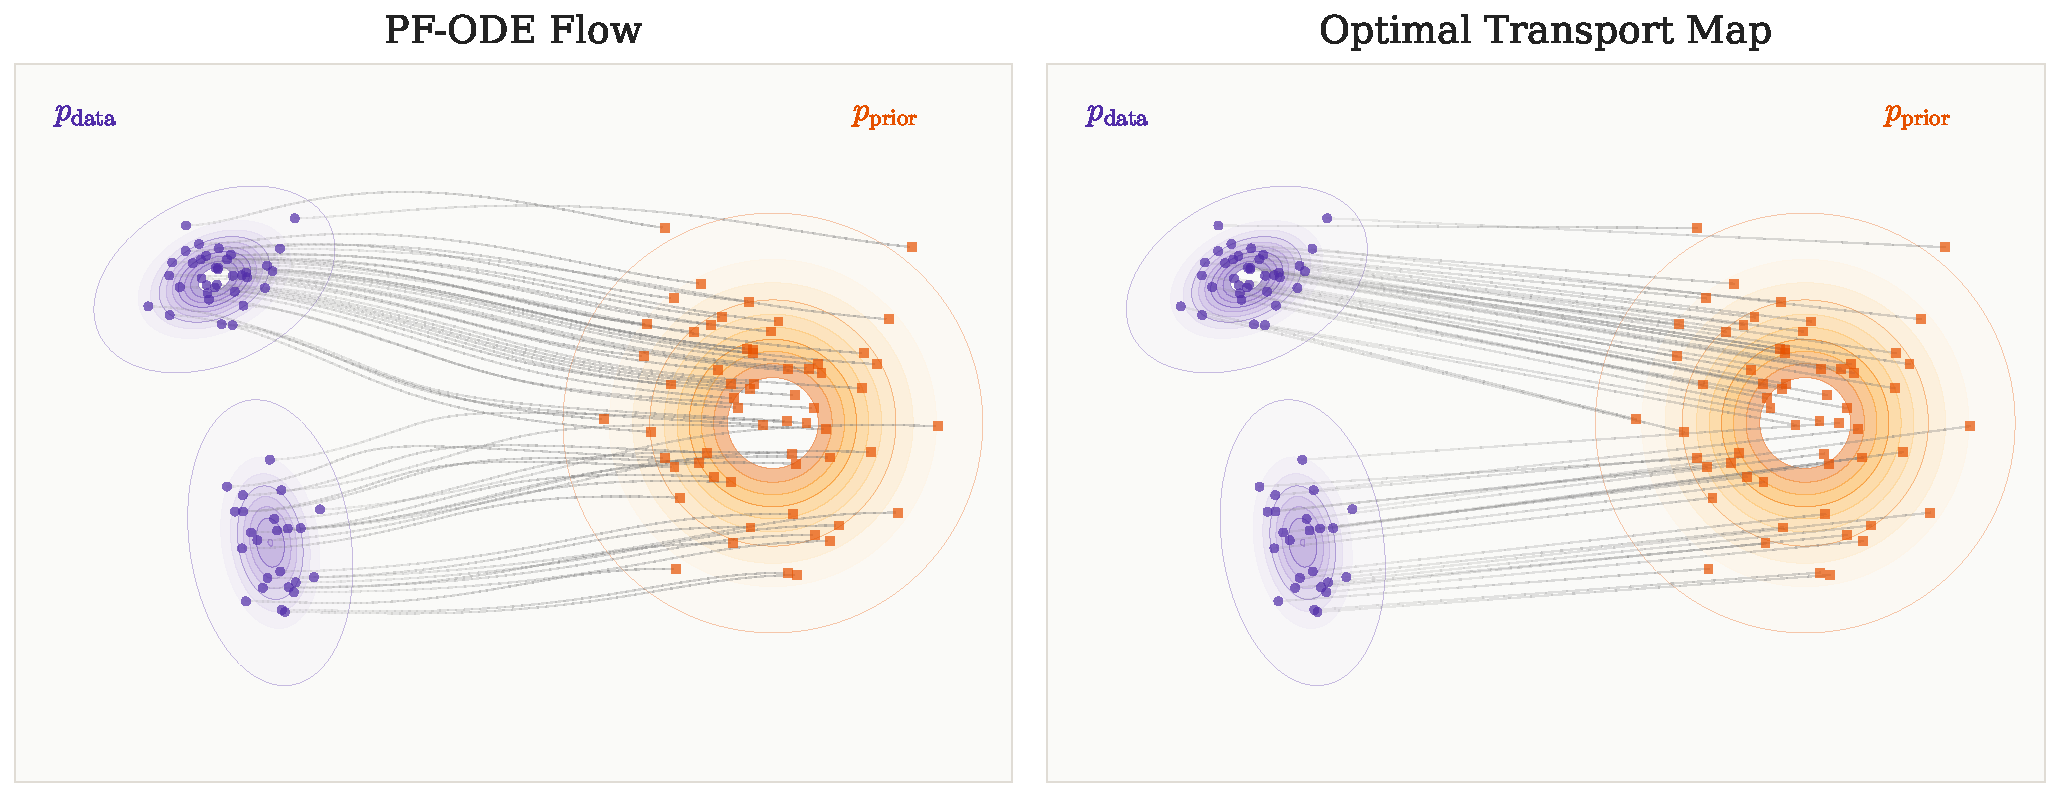
\includegraphics[width=\linewidth]{Images/PartB/pfode_vs_ot_2d.pdf}
    \caption{在二维中比较从 $p_{\mathrm{data}}$ 到 $p_{\mathrm{prior}}$ 的 PF-ODE 流映射与真正的 OT 映射。右：二次代价下的 OT 映射，由匈牙利算法精确计算。左：对 PF-ODE 积分得到的 PF-ODE 流映射。两幅图明显不同，说明 PF-ODE 一般无法还原最优传输映射。
    \figcredit{由作者借助 AI 辅助编码绘制。}}
    \label{fig:pfode-vs-ot-2d}
\end{figure}


\paragraph{设定。} 考虑 VP SDE，具体即 Ornstein--Uhlenbeck 过程，它把光滑的初始密度 $p_0$ 演化趋向标准高斯 $\mathcal{N}(\bm{0}, \rmI)$：
\[
\diff \rvx(t) = -\rvx(t) \diff t + \sqrt{2} \diff \rvw(t), \quad \rvx(0) \sim p_0.
\]
相应的 PF-ODE 为
\[
\frac{\diff \mathbf{S}_t(\rvx)}{\diff t} = -\mathbf{S}_t(\rvx) - \nabla \log p_t(\mathbf{S}_t(\rvx)), \quad \mathbf{S}_0(\rvx) = \rvx.
\]
这里 $\mathbf{S}_t$ 表示把 $p_0$ 前推到边缘 $p_t$ 的流映射：
\[
\left(\mathbf{S}_t\right) \# p_0 = p_t,
\quad\text{即}\quad
p_t(\rvy) = \int_{\mathbb{R}^D} \delta(\rvy - \mathbf{S}_t(\rvx))   p_0(\rvx) \diff \rvx.
\]
这些密度 $p_t$ 按福克尔—普朗克方程演化：
\[
\frac{\partial p_t}{\partial t} = \nabla \cdot (\rvx p_t) + \Delta p_t.
\]
这相当于具有速度场的连续性方程：
\[
\rvv_t(\rvx) = -\rvx - \nabla \log p_t(\rvx),
\]
其流由下式给出 $\mathbf{S}_t(\rvx)$。换句话说，PF-ODE 可以写为：
\[
\frac{\diff \mathbf{S}_t(\rvx)}{\diff t} = \rvv_t\left(\mathbf{S}_t(\rvx)\right).
\]

如 $t \to \infty$，映射将初始分布传输到先验分布：
\[
\mathbf{S}_\infty \# p_0 = \mathcal{N}(\bm{0}, \rmI) =: p_{\text{prior}}.
\]
\paragraph{\citet{lavenant2022flow} 论证的目标。}

\citet{lavenant2022flow} 并不直接判断终端映射 $\mathbf{S}_\infty$ 是否把 $p_0$ 最优地送到高斯分布。他们转而构造了一个特定的初始分布 $p_0$，并考察整条 PF-ODE 轨迹。其核心观察是：最优性可能在流的某个中间时刻就已经失效。他们考虑中间边缘 $p_t = \mathbf{S}_t \# p_0$，并把从 $p_{t_0}$ 到高斯分布的「剩余」传输映射定义为
\[
\mathbf{T}_{t \to \infty} := \mathbf{S}_\infty \circ \mathbf{S}_{t}^{-1}, \quad \text{for all } t\geq 0.
\]
其论证的核心是：对精心选择的 $p_0$，存在某个时刻 $t_0 \geq 0$，使得 $\mathbf{T}_{t_0 \to \infty}$ 并不是把新起点分布 $p_{t_0}$ 以二次代价最优地传输到 $\mathcal{N}(\bm{0}, \rmI)$ 的映射。这一结果表明，PF-ODE 流一般并不给出最优传输映射；而且对某些初始分布，最优性会彻底失效。

\paragraph{预备工具。} \citet{lavenant2022flow} 的论证主要依赖下面这个结果，即 \emph{Brenier 定理}：
\begin{quote}
    \begin{theorem}[Brenier 定理（非正式表述）]\label{thm:brenier}
设 $\nu_1, \nu_2$ 是 $\mathbb{R}^D$ 上两个具有光滑密度的概率分布。光滑映射 $\rmT : \mathbb{R}^D \to \mathbb{R}^D$ 是从 $\nu_1$ 到 $\nu_2$ 的（二次代价下）最优传输映射，当且仅当存在凸函数 $u$ 使 $\rmT = \nabla u$。此时 $\mathrm{D} \rmT$ 对称且半正定，并且 $u$ 满足 Monge--Ampère 方程：
\[
\det \mathrm{D}^2 u(\mathbf{x}) = \frac{\nu_1(\mathbf{x})}{\nu_2(\nabla u(\mathbf{x}))}.
\]
\end{theorem}
\end{quote}

证明中还默认用到下面这个事实，此后不再重复说明：\emph{一个映射是两个分布间的最优传输映射，当且仅当其逆映射是反方向上的最优传输映射。}


\paragraph{证明思路：PF-ODE 一般并不是 OT 映射。} \citet{lavenant2022flow} 采用反证法：假设对每个 $t\ge0$，映射
\[
\mathbf{T}_t  =  \mathbf{S}_t \circ \mathbf{S}_\infty^{-1}
\]
都是 $\mathcal{N}(\bm{0},\rmI)$ 到 $p_t$ 的二次代价最优传输映射。


\subparagraph{第 1 步：Brenier 定理。} 根据 Brenier 定理，从高斯分布出发的最优传输映射，其雅可比矩阵必须对称且半正定。因此
\[
\mathrm{D} \mathbf{T}_t(\rvx) = \mathrm{D} \mathbf{S}_t(\mathbf{S}_\infty^{-1}(\rvx)) \mathrm{D} (\mathbf{S}_\infty^{-1})(\rvx)
\]
必须对一切 $t$ 与 $\rvx$ 都对称。这里 $\mathrm{D} \mathbf{T}_t(\rvx)$ 表示关于 $\rvx$ 的全微分。

\subparagraph{第 2 步：对对称性条件关于时间求导。}
对时间求导得
\[
\frac{\partial}{\partial t} \mathrm{D}\mathbf{T}_t(\rvx)
= \left( \frac{\partial}{\partial t} \mathrm{D} \mathbf{S}_t \right)(\mathbf{S}_\infty^{-1}(\rvx)) \mathrm{D} (\mathbf{S}_\infty^{-1})(\rvx).
\]
既然对称性对一切 $t$ 成立，这个导数也保持对称。利用流所满足的 ODE（对 $\rvx$ 求微分），得到
\[
\frac{\partial (\mathrm{D}\mathbf{S}_t)}{\partial t}
= \mathrm{D}\rvv_t(\mathbf{S}_t) \cdot \mathrm{D}\mathbf{S}_t
= \left( -\rmI - \mathrm{D}^2 \log p_t(\mathbf{S}_t) \right) \cdot \mathrm{D}\mathbf{S}_t.
\]
综合上面两式可见，
\[
\left( -\rmI - \mathrm{D}^2 \log p_t(\mathbf{S}_t) \right) \cdot\mathrm{D}\mathbf{S}_t \cdot \mathrm{D} (\mathbf{S}_\infty^{-1})
\]
对一切 $t\geq 0$ 都对称。取 $t = 0$，此时 $\mathbf{S}_0 = \rmI$、$\mathrm{D}\mathbf{S}_0 = \rmI$，于是
\[
\left( -\rmI - \mathrm{D}^2 \log p_0(\mathbf{S}_\infty^{-1}(\rvx)) \right) \cdot \mathrm{D} (\mathbf{S}_\infty^{-1})(\rvx) \quad \text{is symmetric}.
\]

\subparagraph{第 3 步：交换性条件。} 由于按假设 $\mathbf{T}_0 = \mathbf{S}_\infty^{-1}$ 是最优的，其雅可比矩阵 $\mathrm{D}\mathbf{T}_0 = \mathrm{D}(\mathbf{S}_\infty^{-1})$ 对称。此外 Hessian 矩阵 $\mathrm{D}^2\log p_0$ 也对称。注意：两个对称矩阵的乘积对称，当且仅当二者可交换。因此对一切 $\mathbf{x}\in\mathbb{R}^D$，
\[
\mathrm{D}^2\log p_0\bigl(\mathbf{S}_\infty^{-1}(\mathbf{x})\bigr)
\quad\text{must commute with}\quad
\mathrm{D}(\mathbf{S}_\infty^{-1})(\mathbf{x}) .
\]
令 $\mathbf{y}=\mathbf{S}_\infty^{-1}(\mathbf{x})$，即得等价条件：对一切 $\rvy\in\mathbb{R}^D$，
\[
\mathrm{D}^2\log p_0(\mathbf{y})
\quad\text{must commute with}\quad
\mathrm{D}\mathbf{S}_\infty(\mathbf{y}) .
\]


下面把这个条件转化为更便于计算的形式。由于 $\mathbf{S}_\infty$ 是 $p_0$ 与 $\mathcal{N}(\bm{0},\rmI)$ 之间的最优映射，Brenier 定理保证存在凸函数 $u$ 使 $\mathbf{S}_\infty = \nabla u$。再结合 Monge--Ampère 方程，可得
\[
\log p_0(\rvy) = \log \det(\mathrm{D}^2 u(\rvy)) - \frac{1}{2} \|\nabla u(\rvy)\|^2 + \text{Constant}.
\]
于是条件变为（用到 $\mathrm{D}\mathrm{S}_\infty = \mathrm{D}^2 u$）：
\begin{mdframed}
\begin{align}\label{eq:necessary-ot}
\mathrm{D}^2 \left(\log \det \mathrm{D}^2 u - \frac{1}{2} \|\nabla u\|^2\right)
\quad\text{must commute with}\quad
\mathrm{D}^2 u.
\end{align}
\end{mdframed}
这就给出了 $\mathbf{T}_t$ 为最优映射的一个必要条件。

\subparagraph{第 4 步：构造反例。} 下面说明如何利用这一必要条件导出矛盾。只要能构造出一个凸函数 $u$，使得
\[
\mathrm{D}^2 \left( \log \det \mathrm{D}^2 u(\mathbf{x}) - \frac{1}{2} \lvert \nabla u(\mathbf{x}) \rvert^2 \right)
\]
对某些 $\mathbf{x} \in \mathbb{R}^D$ 不与 $\mathrm{D}^2 u(\mathbf{x})$ 可交换即可。令 $p_0 = (\nabla u)^{-1} \# \mathcal{N}(\bm{0}, \rmI)$，由 Brenier 定理，$\nabla u$ 就是从 $p_0$ 到 $\mathcal{N}(\bm{0}, \rmI)$ 的最优映射。但此时 \Cref{eq:necessary-ot} 中的条件不成立，矛盾即导出。因此我们的目标就是构造这样的函数。考虑
\[
u(\mathbf{x}) = \frac{1}{2} \|\mathbf{x}\|^2 + \varepsilon \phi(\mathbf{x}), \quad \text{（$\varepsilon$ 取小量）}.
\]
于是 $\mathrm{D}^2 u(\mathbf{0}) = \rmI + \varepsilon \mathrm{D}^2 \phi(\mathbf{0})$，而 $\mathbf{x} = \mathbf{0}$ 处的交换性条件要求 $\mathrm{D}^2 \phi(\mathbf{0})$ 与 $\mathrm{D}^2 (\Delta \phi)(\mathbf{0})$ 可交换。例如在 $\mathbb{R}^2$ 中，取
\[
\phi(x_1, x_2) = x_1 x_2 + x_1^4
\]
即构成一个反例：此时 Hessian 矩阵 $\mathrm{D}^2 \log p_0$ 与雅可比矩阵 $\mathrm{D}^2 u$ 不可交换。这一矛盾说明 $\mathbf{T}_t$ 不可能对一切 $t \geq 0$ 都是最优的；于是必有某个 $t_0 \geq 0$，使映射 $\mathbf{T}_{t_0 \to \infty}$ 不再最优。


\subsection{标准线性流与 reflow 能否生成 OT 映射？}\label{subsec:ot-linear-reflow}
我们已经看到，PF-ODE（尤其是 VP 型前向核）通常并不给出 OT 映射。于是自然要问：
\begin{question}
如果把线性插值流 $(1-t)\rvx_0 + t \rvx_1$（其中 $\rvx_0\sim p_{\mathrm{src}}$、$\rvx_1\sim p_{\mathrm{tgt}}$）用在独立耦合上，即 $\pi(\rvx_0, \rvx_1) = p_{\mathrm{src}}(\rvx_0)p_{\mathrm{tgt}}(\rvx_1)$，能否还原 OT 映射？
\end{question}
答案是「不能」。不过，把线性路径与给定耦合结合起来，可以给出真实 OT 代价的一个实际上界；而在所有可能的路径中，线性插值给出的上界是最紧的，下面的讨论将说明这一点。


\paragraph{规范线性流与最优传输。}
对于二次代价下的最优传输，我们考察 \Cref{eq:ot} 的如下等价形式，即 Benamou--Brenier 表述 \Cref{eq:bb-ot}：
\begin{equation*}
    \mathcal{K}\left(p_{\mathrm{src}}, p_{\mathrm{tgt}}\right) :=  \min_{\substack{ (p_t, \rvv_t) \text{ s.t. }
        \partial_t p_t + \nabla \cdot (p_t \rvv_t) = 0, \\
        p_0 = p_{\mathrm{src}},\,\, p_1 = p_{\mathrm{tgt}}
    }}
    \int_0^1 \int_{\mathbb{R}^D} \|\rvv_t(\rvx)\|^2 p_t(\rvx) \diff\rvx \diff t.
\end{equation*}
与静态的 Monge 表述不同（\Cref{eq: Monge's Formulation}；那里求最优映射需要解 Monge--Ampère 方程，见 \Cref{eq:monge-ampere}），Benamou--Brenier 问题在引入动量场
$\rvm_t := p_t \rvv_t$ 之后具有凸的重构形式。尽管如此，要在 $\mathbb{R}^D$ 的网格上离散化这个凸问题，在高维情形下依然难以处理。虽然求解 Benamou--Brenier 表述通常很棘手，但 \citet{liu2022rectified,lipman2024flow} 指出其动能存在一个实用的上界。其做法是把搜索范围限制在更简单的一族\emph{条件流}中：每一条路径都由它的固定端点 $(\rvx_0, \rvx_1)$ 确定，而端点对由源分布与目标分布之间的耦合 $\pi_{0,1}$ 诱导。在\emph{条件流}这一族里，规范线性插值就是最优选择，如下所示。

\proppp{用条件流给出 OT 动能的上界}{ot-conditional-flow}{
设 $\pi_{0,1}$ 为 $p_{\mathrm{src}}$ 与 $p_{\mathrm{tgt}}$ 之间的任一耦合。
\begin{enumerate}
    \item[(1)] 动能不超过任一连接两端的条件流 $\bm{\Psi}_t(\rvx_0, \rvx_1)$ 的期望路径能量：
    \begin{equation*}
        \mathcal{K}\left(p_{\mathrm{src}}, p_{\mathrm{tgt}}\right) \le \mathbb{E}_{(\rvx_0, \rvx_1) \sim \pi_{0,1}} \left[ \int_0^1 \|\bm{\Psi}'_t(\rvx_0, \rvx_1)\|^2 \diff t \right].
    \end{equation*}
    \item[(2)] 使右端上界取到最小的那个唯一的条件流 $\bm{\Psi}^*_t$，正是线性插值路径：
    \begin{equation*}
        \bm{\Psi}^*_t(\rvx_0, \rvx_1) = (1 - t) \rvx_0 + t \rvx_1.
    \end{equation*}
  将其代回，即得最紧的上界：
    \begin{equation*}
        \mathcal{K}\left(p_{\mathrm{src}}, p_{\mathrm{tgt}}\right) \le \mathbb{E}_{(\rvx_0, \rvx_1) \sim \pi_{0,1}} \|\rvx_1 - \rvx_0\|^2.
    \end{equation*}
\end{enumerate}
}{证明依赖于 Jensen 不等式与条件期望的塔性质的直接运用，之后再用 Euler--Lagrange 方程求解化简后的变分问题；完整论证参见 \citet{lipman2024flow} 第 4.7 节。}

换句话说，线性插值 $\bm{\Psi}^*_t$（也就是流匹配与整流流所采用的前向转移核）使任一固定耦合 $\pi_{0,1}$ 下真实动能的上界取到最小。

需要强调的是：在条件流这一族内部取到最优，并不能保证边缘分布在全局意义上也是最优的。


\paragraph{Reflow 与最优传输。}
两个分布之间最朴素的传输方案，是用最简单的独立耦合把它们的样本用直线两两连起来。但这种方法显然不是最优的：问题并不出在直线路径本身，而出在初始点对的配对方式太粗糙。Reflow 流程可以对此作出建设性的回应。它是一个专门为纠正这种配对而设计的迭代算法，而且最重要的是，它保证每一步的代价都不会增加 \citep{liu2022flow}。这一性质说明 Reflow 会系统地把传输方案推向更优的配置，于是自然引出一个关于收敛性的核心问题。
\begin{question}
    反复施加 \texttt{Rectify} 这一迭代算子会发生什么？所得的传输方案序列会收敛到最优方案吗？或者说，reflow 流程的不动点会不会给出 OT 映射？
\end{question}
简短的回答是：一般不会。下面我们解释可能出现的问题。回顾一下，reflow 通过如下更新来迭代地改进 $p_{\mathrm{src}}$ 与 $p_{\mathrm{tgt}}$ 之间的耦合：
\[
\pi^{(k+1)} = \texttt{Rectify}(\pi^{(k)}),
\]
并以乘积耦合 $\pi^{(0)} := p_{\mathrm{src}}(\rvx_0) p_{\mathrm{tgt}}(\rvx_1)$ 初始化。更具体地说，$\texttt{Rectify}$ 按下述方式输出更新后的耦合 $\pi^{(k+1)}$：在第 $k = 0, 1, 2, \ldots$ 轮迭代中，先学习速度场 $\rvv_t^{(k)}$
\[
\rvv_t^{(k)} \in \argmin_{\rvu_t} \, \mathcal{L}(\rvu_t\big\vert\pi^{(k)}),
\]
其中 $\mathcal{L}(\rvu_t\big\vert\pi^{(k)})$ 是 \Cref{eq:reflow-loss} 中定义的损失（例如 RF 或 FM 损失）。这里为记号简便，我们对速度场采用非参数写法，而不用其他处所用的参数化形式 $\bm{\phi}$。更新后的耦合则由下式给出：
\[
\pi^{(k+1)}(\rvx_0, \rvx_1) := p_{\mathrm{src}}(\rvx_0)\, \delta\big(\rvx_1 - \bm{\Psi}_1^{(k)}(\rvx_0)\big),
\]
其中 $\bm{\Psi}_1^{(k)}$ 表示以 $\rvx_0$ 为初值、对 $\rvv_t^{(k)}$ 积分到 $t=1$ 所得的解映射。\citet{liu2022flow} 观察到：对于 $p_{\mathrm{src}}$ 与 $p_{\mathrm{tgt}}$ 之间的耦合 $\pi$，存在使 reflow 损失最小的速度场 $\rvv_t$（即满足 $\mathcal{L}(\rvv_t |\pi) = 0$），并不一定意味着该传输是最优的。受 Benamou--Brenier 框架的启发（该框架下最优传输速度已知是某个势函数的梯度），\citet{liu2022rectified} 追加了一条约束：速度场 $\rvv_t$ 应当是一个势场。于是把 \Cref{eq:reflow-loss} 的目标改为只在梯度向量场（也称势流）空间中搜索 $\rvv_t$：
\begin{align}\label{eq:reflow-loss-gradient}
    \rvw_t^{(k)} \in \argmin_{\substack{\rvu_t:\, \rvu_t=\nabla\varphi \\ \text{for some }\varphi\colon\mathbb{R}^D\to\mathbb{R}}} \, \mathcal{L}(\rvu_t\big\vert\pi^{(k)}),
\end{align}
其余步骤与 \texttt{Rectify} 相同。我们把这一关联算子记为 $\texttt{Rectify}_{\perp}$，以强调它是向无旋向量场的投影。设 $\pi$ 为 $p_{\mathrm{src}}$ 与 $p_{\mathrm{tgt}}$ 之间的耦合，\citet{liu2022flow} 猜想下述条件等价于最优性：
\begin{enumerate}[label=(\textit{\roman*})]
  \item $\pi$ \textit{是一个最优传输耦合；}
  \item $\pi$ \textit{是势整流算子的不动点：}
  \[
    \pi = \texttt{Rectify}_{\perp}(\pi).
  \]
  \item \textit{存在梯度速度场 $\rvv_t = \nabla \varphi_t$，使整流损失降为零：}
  \[
    \mathcal{L}(\rvv_t |\pi) = 0.
  \]
\end{enumerate}
然而，\citet{hertrich2025relation} 给出了两类反例：
\begin{enumerate}
  \item 当中间分布 $p_t$ 的支撑不连通时，可以找到 $\texttt{Rectify}_{\perp}$ 的不动点：其 reflow 损失为零、速度场是梯度场，却仍无法给出最优耦合。
  \item 即便两个端点分布都是高斯分布，也存在这样的耦合：其损失可以任意小，而与最优耦合的偏差却可以任意大。
\end{enumerate}

因此，尽管整流流能够产生强大的生成模型，它作为最优传输求解器的可靠性仍然有限。这暴露出生成模型与严格的最优传输理论之间一处重要的空白，也促使人们进一步研究两者的交叉地带。

最后需要指出，传输代价并不总与下游表现相关；因此，算出精确的最优传输映射，未必一定带来更好的实际效果。尽管如此，最优传输的各种变体仍然是科学与工程中许多问题的基石，而扩散模型则为探索这些挑战提供了一个强有力的框架。

\section{结束语}
本章重新审视了「把一个分布搬运成另一个分布」这一经典问题，并通过最优传输及其熵变体的视角来考察它。我们回顾了静态最优传输的
Monge--Kantorovich 形式，以及其动态的 Benamou--Brenier 表述——在其中传输由一条使动力学代价最小的确定性流来实现。接着我们讨论了熵正则化最优传输与薛定谔桥（SB）：后者借助相对于参考过程「最可能」的受控扩散来刻画传输。从这一角度看，扩散模型在随机这一侧自然落在 SB 观点附近，
而其 PF-ODE 则在 ODE 这一侧定义了确定性的传输映射。然而正如我们所强调的，PF-ODE 给出的
传输通常\emph{并不是}二次代价下的最优传输
映射：它只是众多确定性耦合中的一种，而并不
使 Benamou--Brenier 作用量最小。这也引出一个更基本的问题：在追问某个传输是否最优之前，\emph{究竟什么时候可以用一个确定性映射把两个分布连接起来？} 在许多设定中，「存在性」并不是主要的
困难。在适当的正则性假设下，通常都能找到可测映射 $\rmT$ 使
$\rmT_\# p_{\mathrm{src}} = p_{\mathrm{tgt}}$。更难的问题在于：
一旦超出一维，兼具显式表达与实用稳健性的经典结构就相对少见。在一维情形，单调重排通过匹配分位数给出了一个简洁的答案。在更高维，已知的重要结构只有少数几个：Brenier 定理
（定理~\ref{thm:brenier}）在适当正则性下给出二次代价的最优映射；Knott--Rosenblatt
重排~\citep{rosenblatt1952remarks,knothe1957contributions}
通过迭代条件分布构造出三角映射；以及
Dacorogna--Moser 方法~\citep{dacorogna1990partial}，它通过求解散度方程得到速度场，进而构造光滑的微分同胚传输。这些都给确定性传输提供了有原则的途径，但每一个都依赖结构性的假设或相当繁重的分析工具。

从这个角度看，基于扩散的流映射提供了一个有吸引力且灵活的替代方案。扩散模型与流匹配方法并不预设一个闭式的传输映射，而是学习一个依赖时间的向量场，由其诱导的流把简单的源分布推向目标分布。这样学到的映射不必与 Brenier
映射或任何其他经典规范结构相重合，一般来说它也并不求解某个给定的最优传输问题。尽管如此，它提供了一条实用且表达力强的、基于映射的采样途径，适用于那些显式传输映射结构通常不可得、或难以计算的维度。在这个意义上，扩散流最好不要理解成经典传输理论的替代品，而应看作一种现代的可学习传输机制，与最优传输映射、三角重排以及基于偏微分方程的构造一同归入更广泛的确定性传输领域。
